\documentclass[a4paper,11pt]{ctexart}

\input{./Header.Tex}

% 部分使用说明
% \begin{lstlisting}[language={C}]
% 正式代码在此输入
% \end{lstlisting}

% \begin{codebox}
% 伪代码在此输入
% \end{codebox}

\begin{document}

\begin{titlepage}
\begin{center}

% 页面正中央插入的图片及哈尔滨工业大学英文全称

\includegraphics[width=0.8\textwidth]{./images/HIT.eps}\\[1cm]
\textsc{\LARGE Harbin Institute of Technology}\\[1.5cm]

% 标题
\hrulefill \\[0.4cm]
{ \huge \bfseries 数字逻辑大作业}\\[0.4cm]
\hrulefill \\[1.5cm]

% 作者和其他信息
\begin{minipage}{0.4\textwidth}
\begin{flushleft} \large

\end{flushleft}
\end{minipage}

% 右侧
\begin{minipage}{\textwidth}
\begin{flushright} \large
\emph{成员A:}冯云龙\\
\emph{学号:}1160300202\\
\emph{成员B:}赖\ \ \ 昕\\
\emph{学号:}1160300203\\
\end{flushright}
\end{minipage}

\vfill
{\large \today}% 底部插入当日日期
\end{center}
\end{titlepage}

\part*{摘要}大作业是在学完本门课程后,对所学知识的综合性考察. 知识覆盖面宽,实验所需时间长。要求学生灵活运用学过的计数器、触发器、译码电路等方面的知识,独立完成从设计、选片、连线、调试、排除故障到实现一个数字系统的全过程,详细书写项目报告。通过综合设计性实验,培养学生灵活运用所学知识解决比较复杂的实际问题的能力。
\paragraph{关键词:电子密码锁}

\tableofcontents            % 生成目录并隔开正文
\newpage

\part{正文}
\section{设计目的及要求}
\begin{enumerate}
\item 设计一个开锁密码至少为4位数字(或更多)的密码锁。
\item 当开锁按键输入代码等于所设密码时启动开锁控制电路,并且用绿灯亮、红灯灭表示开锁状态。
\item 从第一个按扭触动后的5秒内若未能将锁打开,则电路自动复位并发出报警信号,同时用绿灯灭、红灯亮表示关锁状态。
\item 密码锁中的密码可以修改,最高7位。
\item 记录按键次数并显示。
\item 输入密码倒计时。
\end{enumerate}

\section{工作原理、系统方框图}
\begin{center}
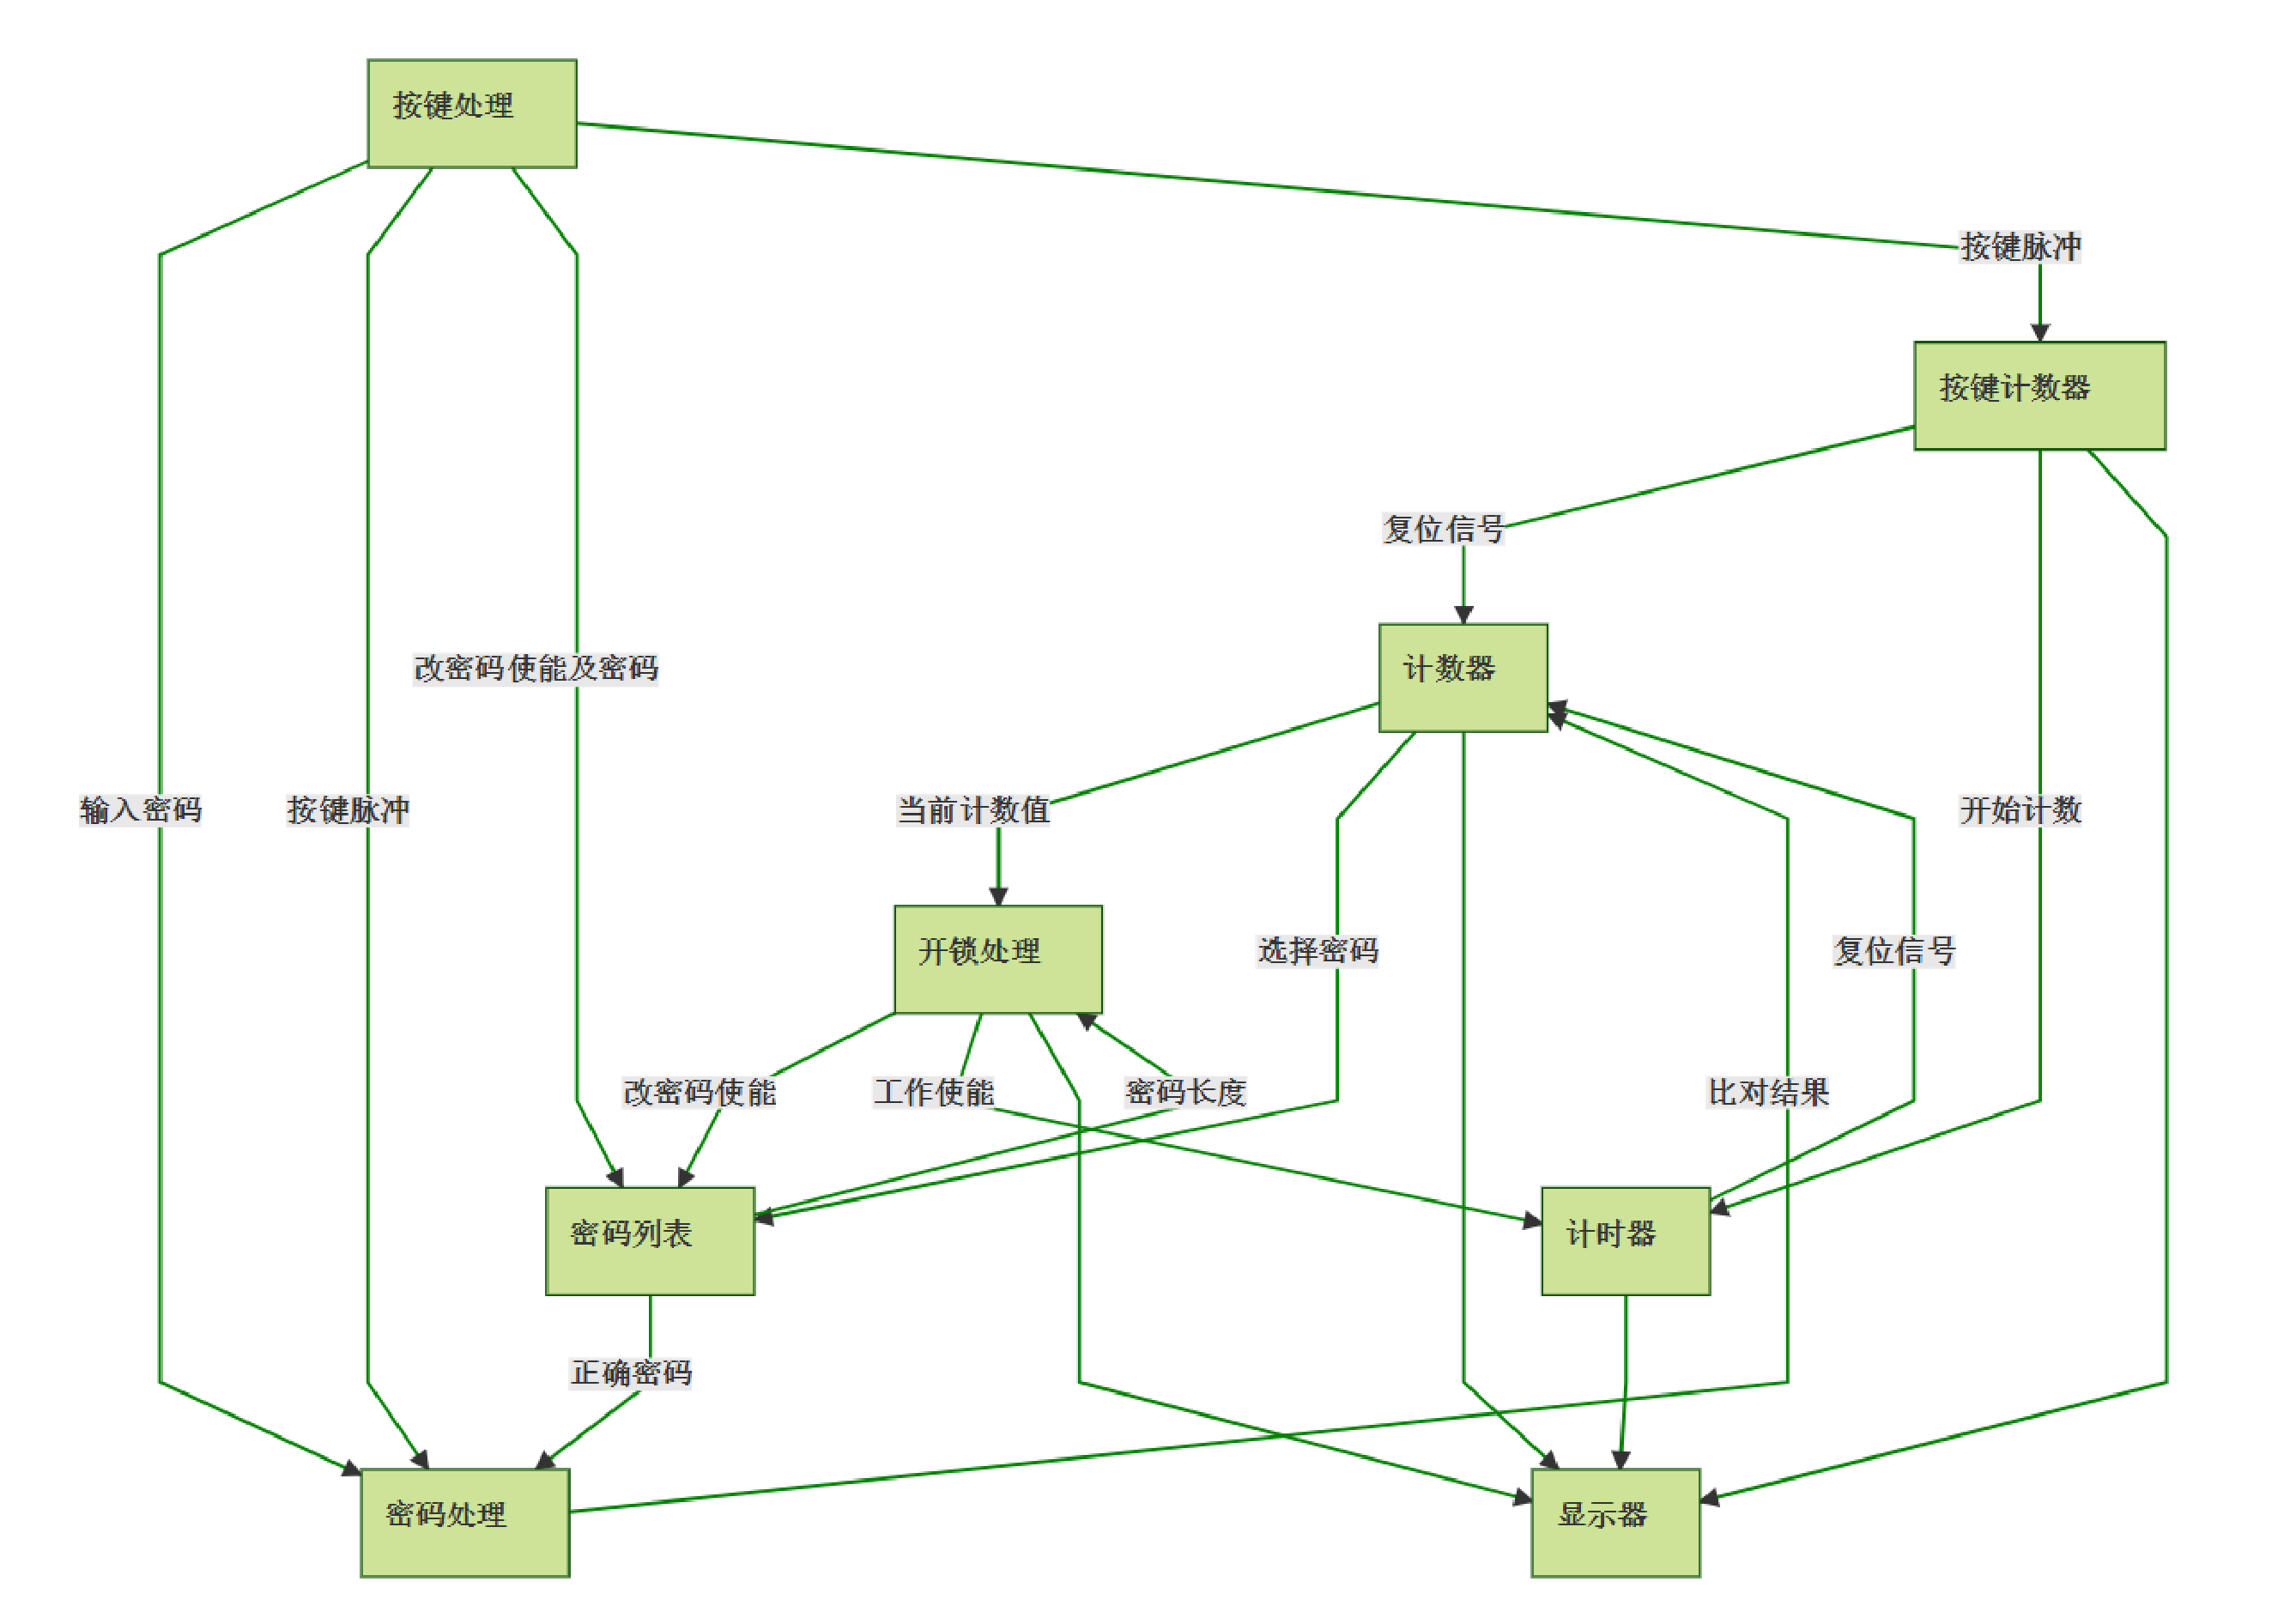
\includegraphics[width=0.9\textwidth]{./images/struct.eps}
\end{center}
\section{各部分选定方案及电路组成、相关器件}
\subsection{密码处理}
\subsubsection{选定方案}这部分我们使用的是一个等值比较器,对密码进行比对,当输入的密码与存储列表中的密码相等时,输出给计数器,使计数器计数。
\subsubsection{电路组成}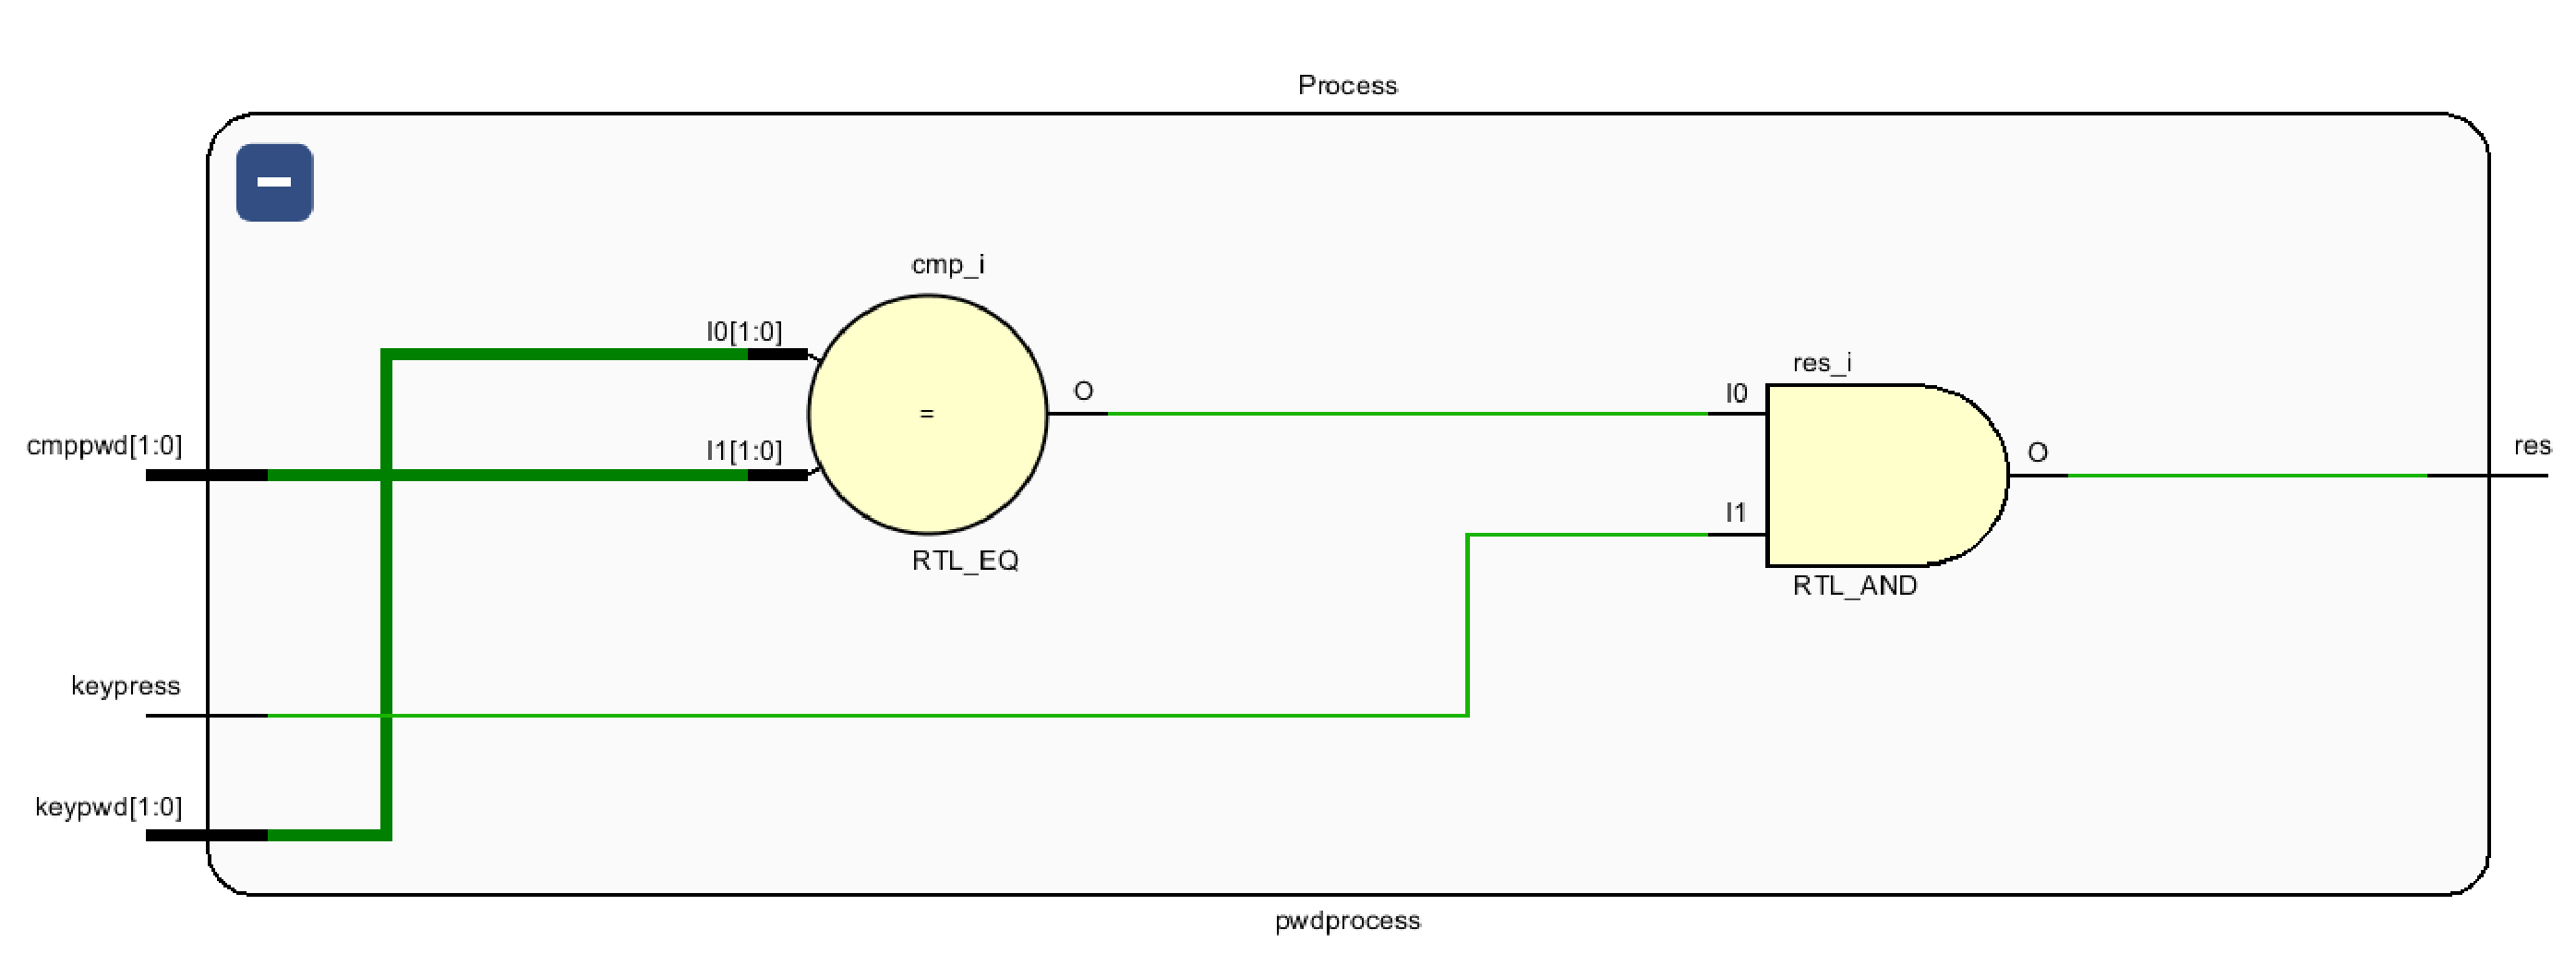
\includegraphics[width = 0.9\textwidth]{./images/ProcessRTL.eps}
\subsubsection{相关器件}等值比较器,逻辑与门。

\subsection{密码表}
\subsubsection{选定方案}首先我们使用了16位寄存器以储存密码和密码长度,使用数据选择器对数据进行选择,在开锁情况下,给予修改信号可以对密码进行修改,当使用计数器对每一位进行修改,可以通过关闭修改信号以停止修改,当不再修改密码时,自动复位。
\subsubsection{电路组成}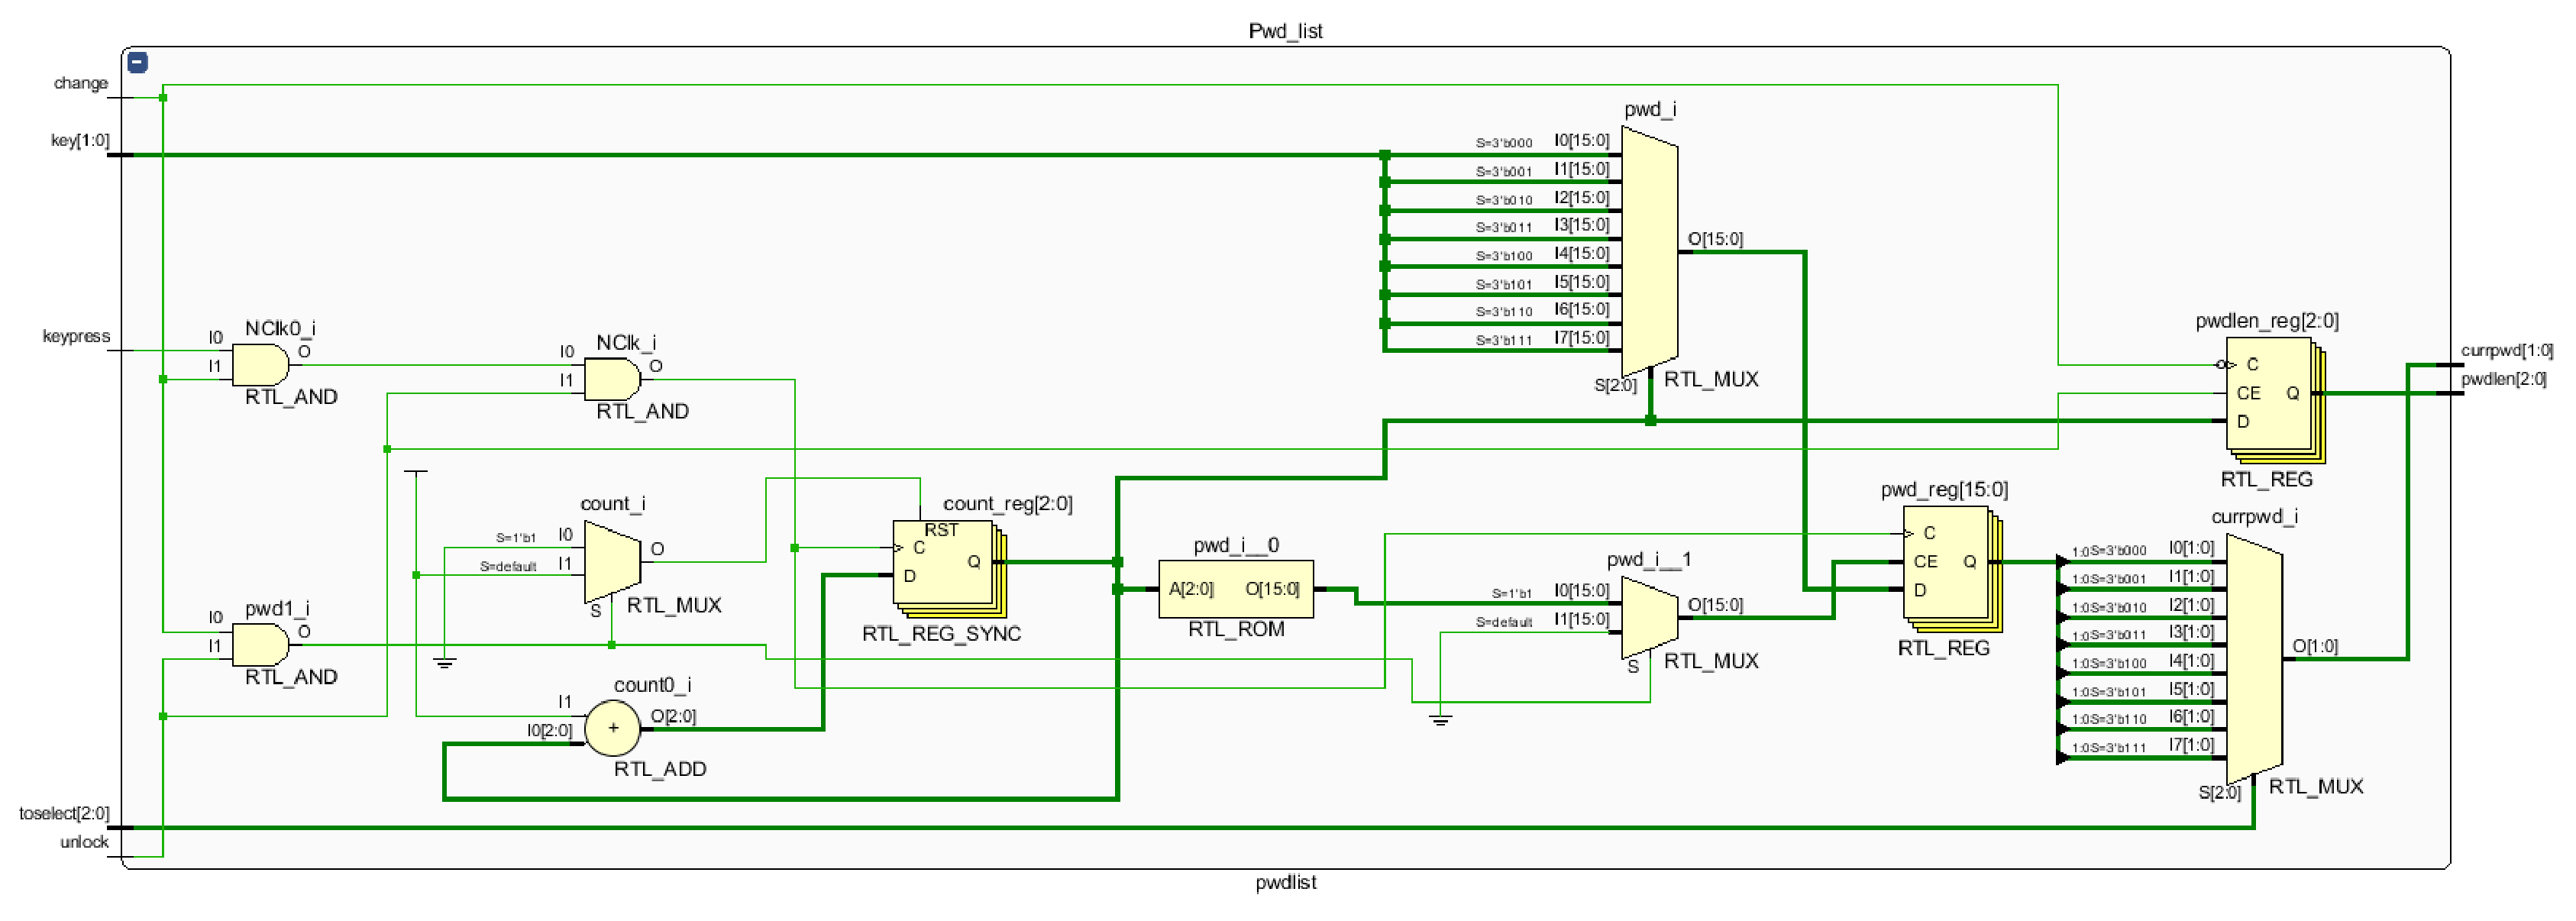
\includegraphics[width = 0.9\textwidth]{./images/PwdlistRTL.eps}
\subsubsection{相关器件}逻辑与门,逻辑非门,加法器,D触发器,数据选择器。

\subsection{密码计数器}
\subsubsection{选定方案}串行输入密码,每输对一位密码,计一次数,可以通过按键计数器与计时器所给的复位信号进行复位(同步清零)。
\subsubsection{电路组成}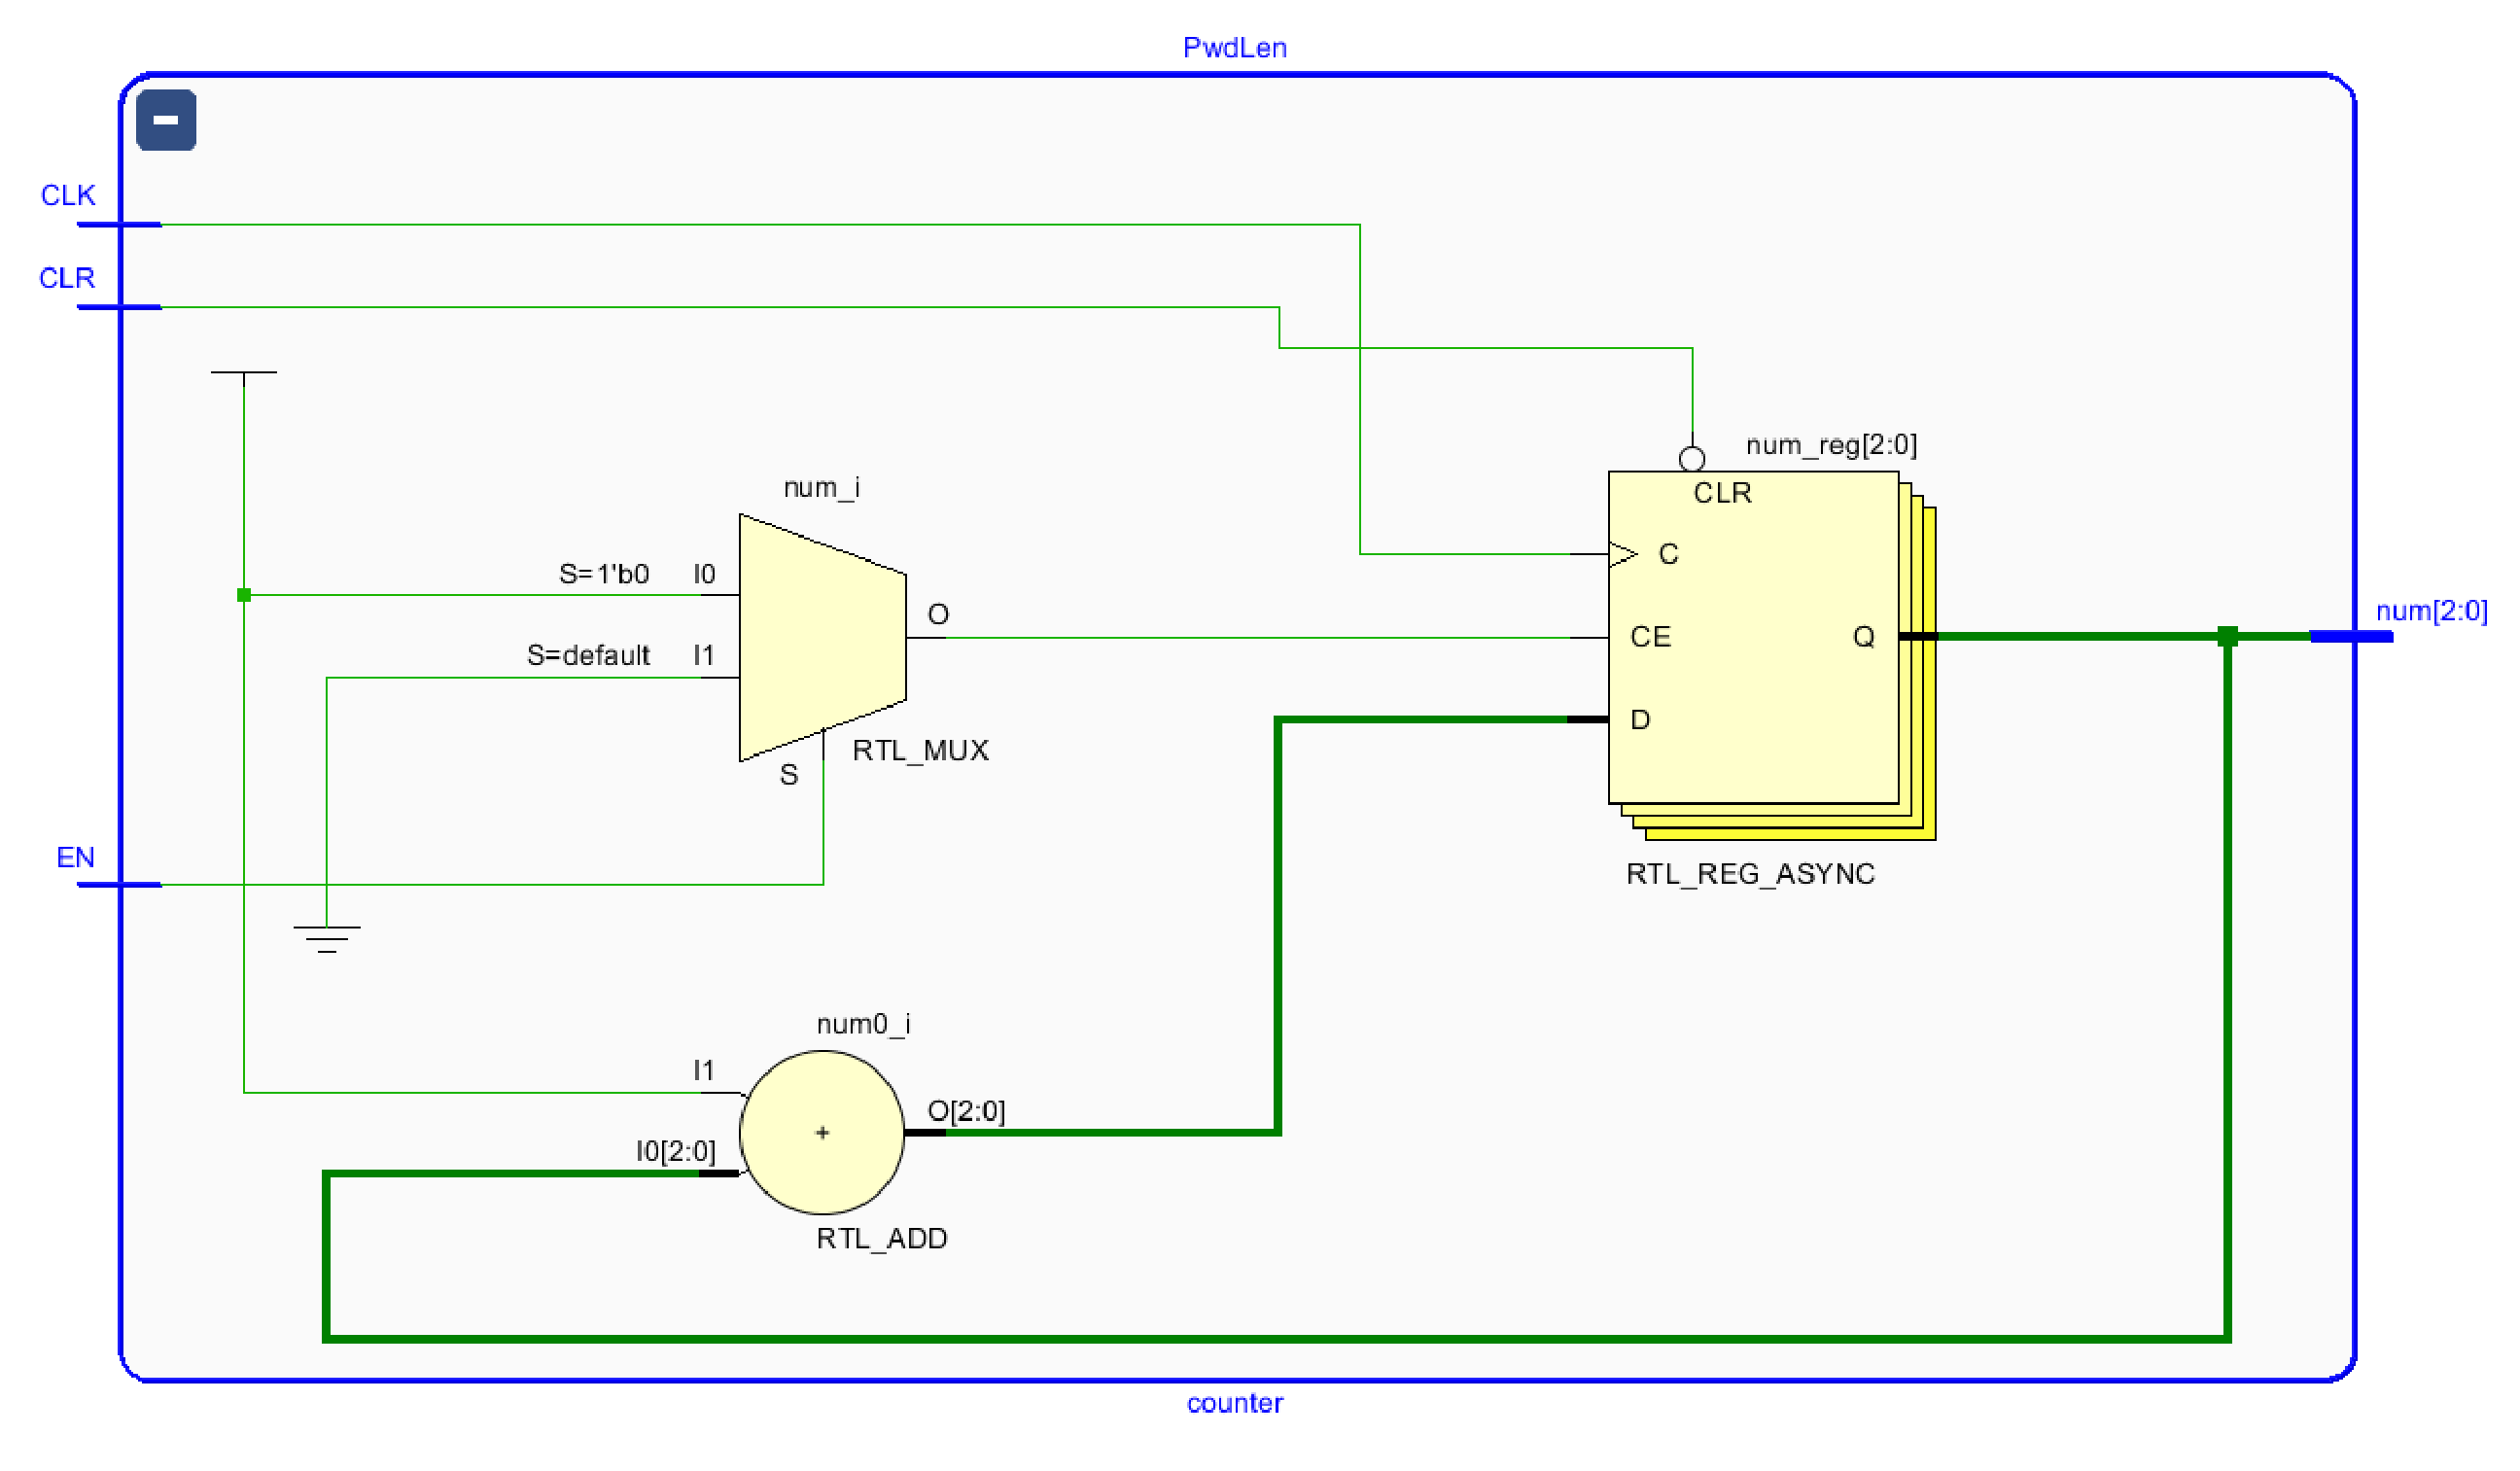
\includegraphics[width = 0.9\textwidth]{./images/PwdLenRTL.eps}
\subsubsection{相关器件}D触发器,加法器,数据选择器。

\subsection{开锁控制器}
\subsubsection{选定方案}实际上是一个等值比较器,将密码计数器的值与设置的密码长度进行比较,若相等,则输出为1。
\subsubsection{电路组成}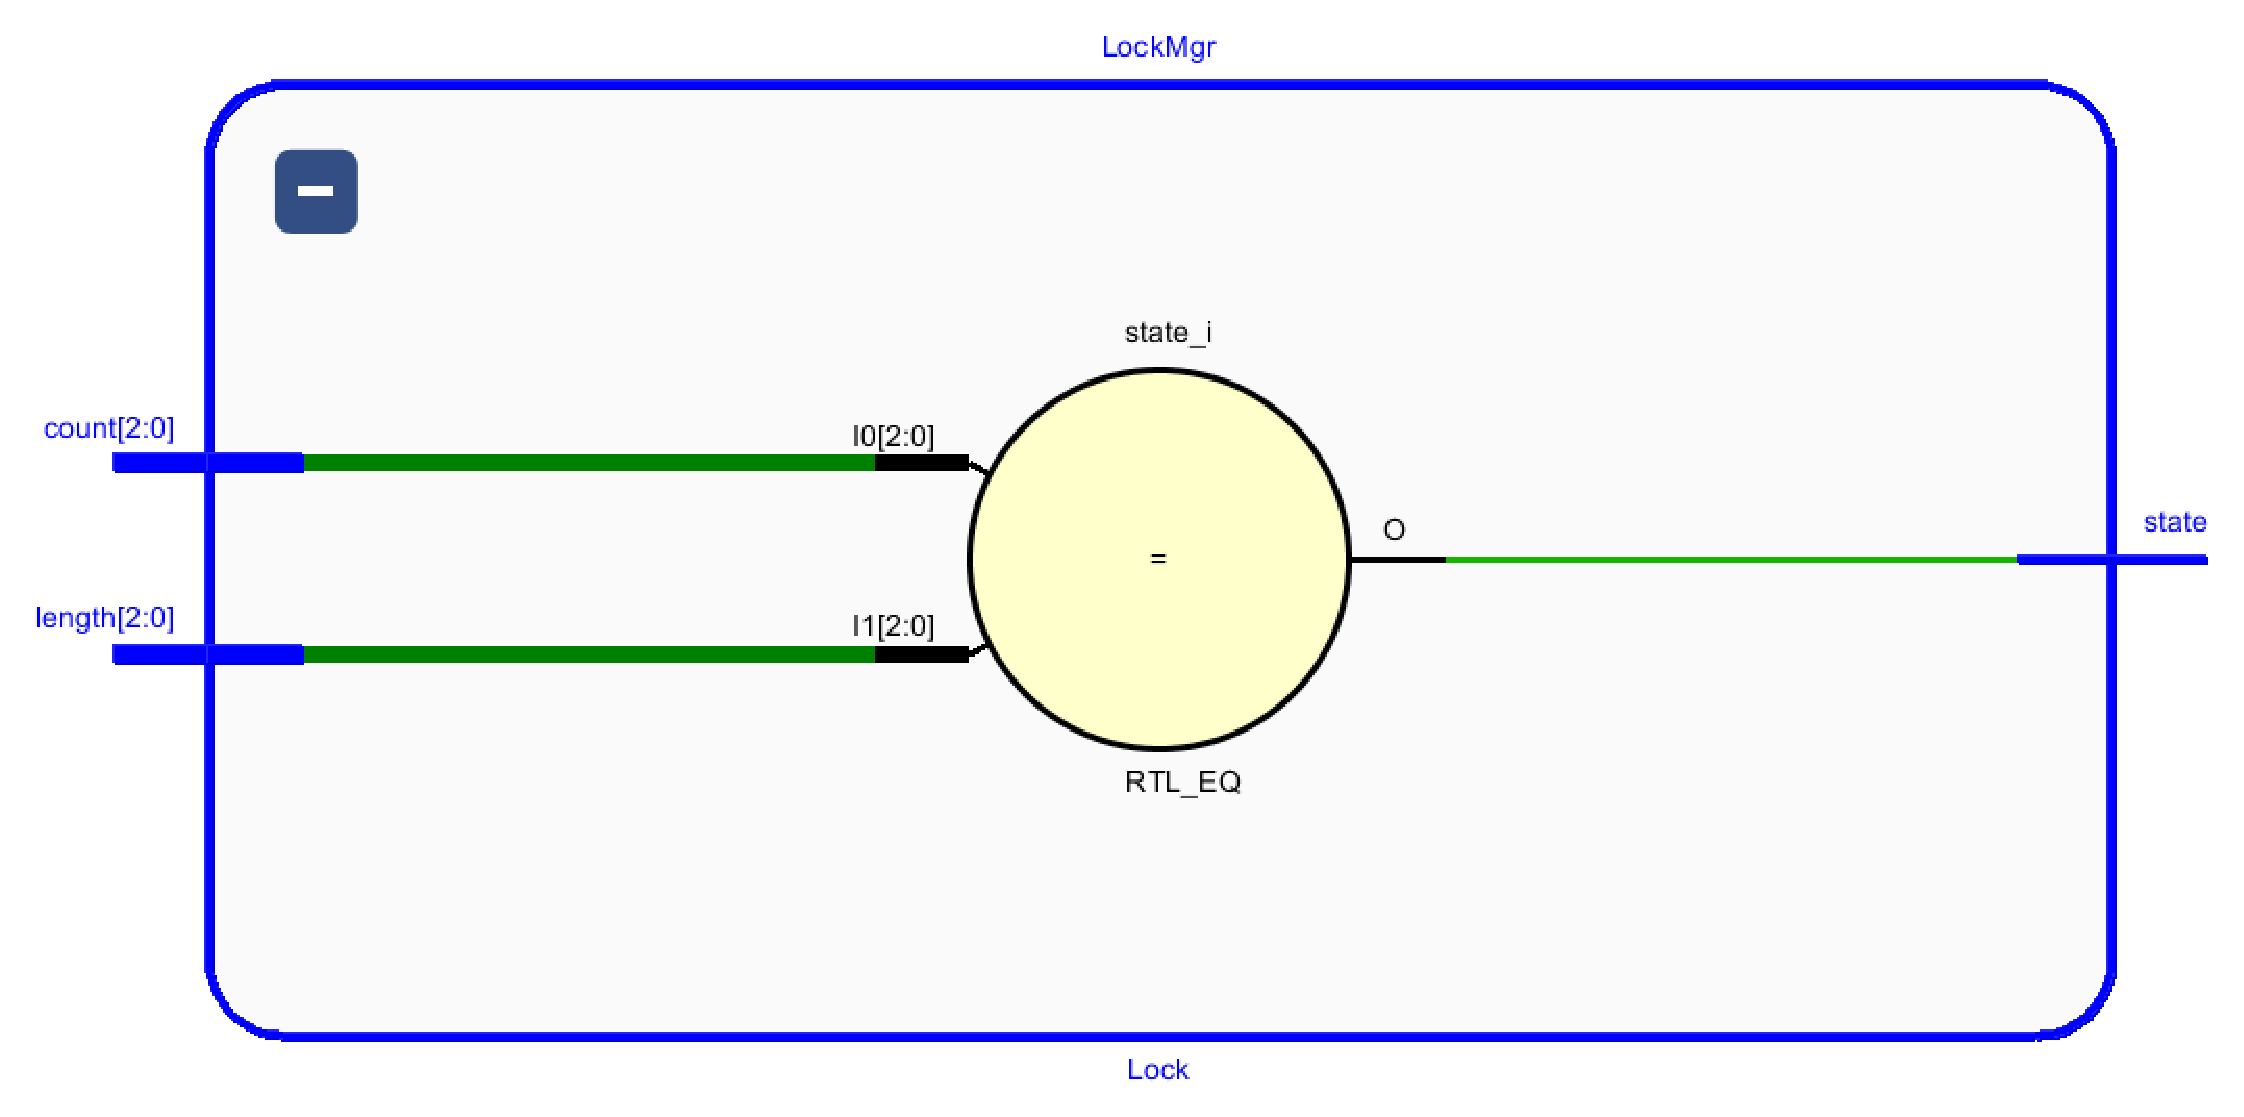
\includegraphics[width =0.9\textwidth]{./images/LockMgrRTL.eps}
\subsubsection{相关器件}等值比较器。

\subsection{核心功能}就是对开锁,解锁,修改密码的整合。
\subsection{计时器}产生倒计时并可以输出倒计时归零信号。
\subsubsection{选定方案}带有计数进位,清零端的计数器。
\subsubsection{相关器件}七段数码管。

\subsection{按键处理}
\subsubsection{选定方案}以一个4-2编码器为基础进行改进。通过一个控制端对输出进行选择出口;并且设计了2个时钟输出端,其中一个给按键计数器,另外一个给密码处理;由于存在险象竞争,故给密码处理的时钟稍微比按键脉冲稍微延迟一些。延迟器可利用一个移位寄存器实现。
\subsubsection{电路组成}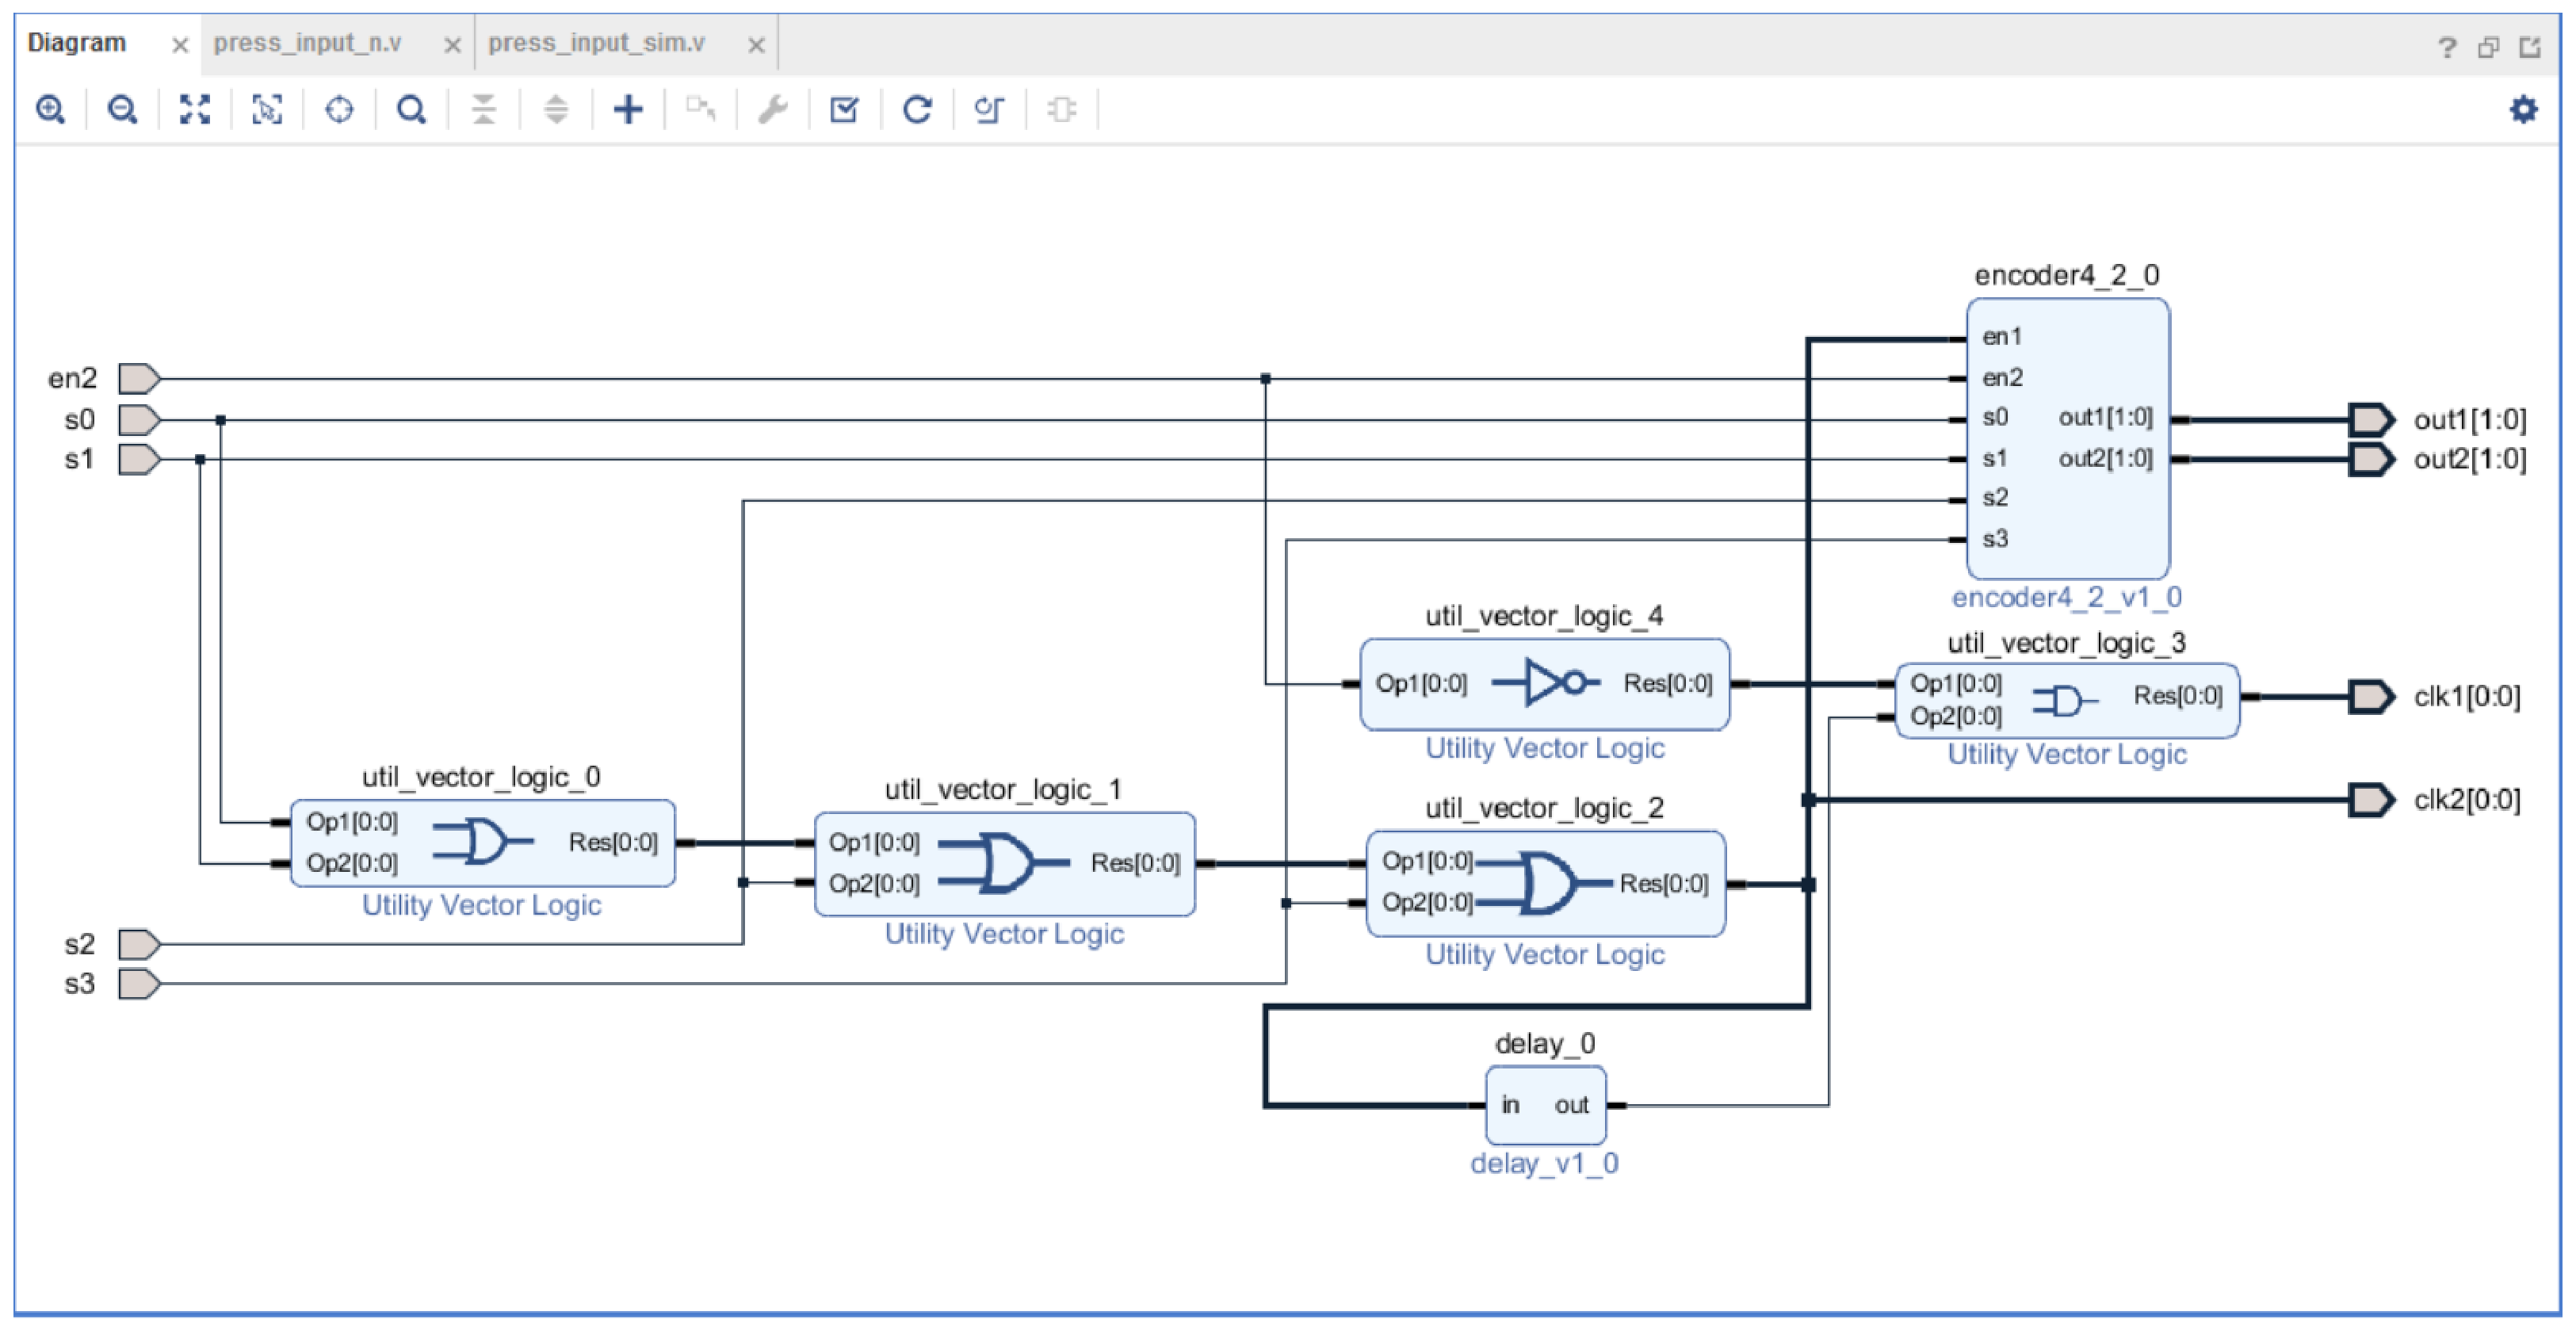
\includegraphics[width =0.9\textwidth]{./images/pic4.eps}
\subsubsection{相关器件}4-2编码器,移位寄存器。

\subsection{按键计数器}
\subsubsection{选定方案}以一个模8计数器为基础进行改进。计数器当前数值即当前输入密码的位数。并在此基础上设计了2个输出端。其中一个输出信号当按下第一个键后一直为1,这个信号用来作为计时器的计时开始输入端;另一个当计数满8时为1,这个信号用来作为给计数器的复位信号。
\subsubsection{电路组成}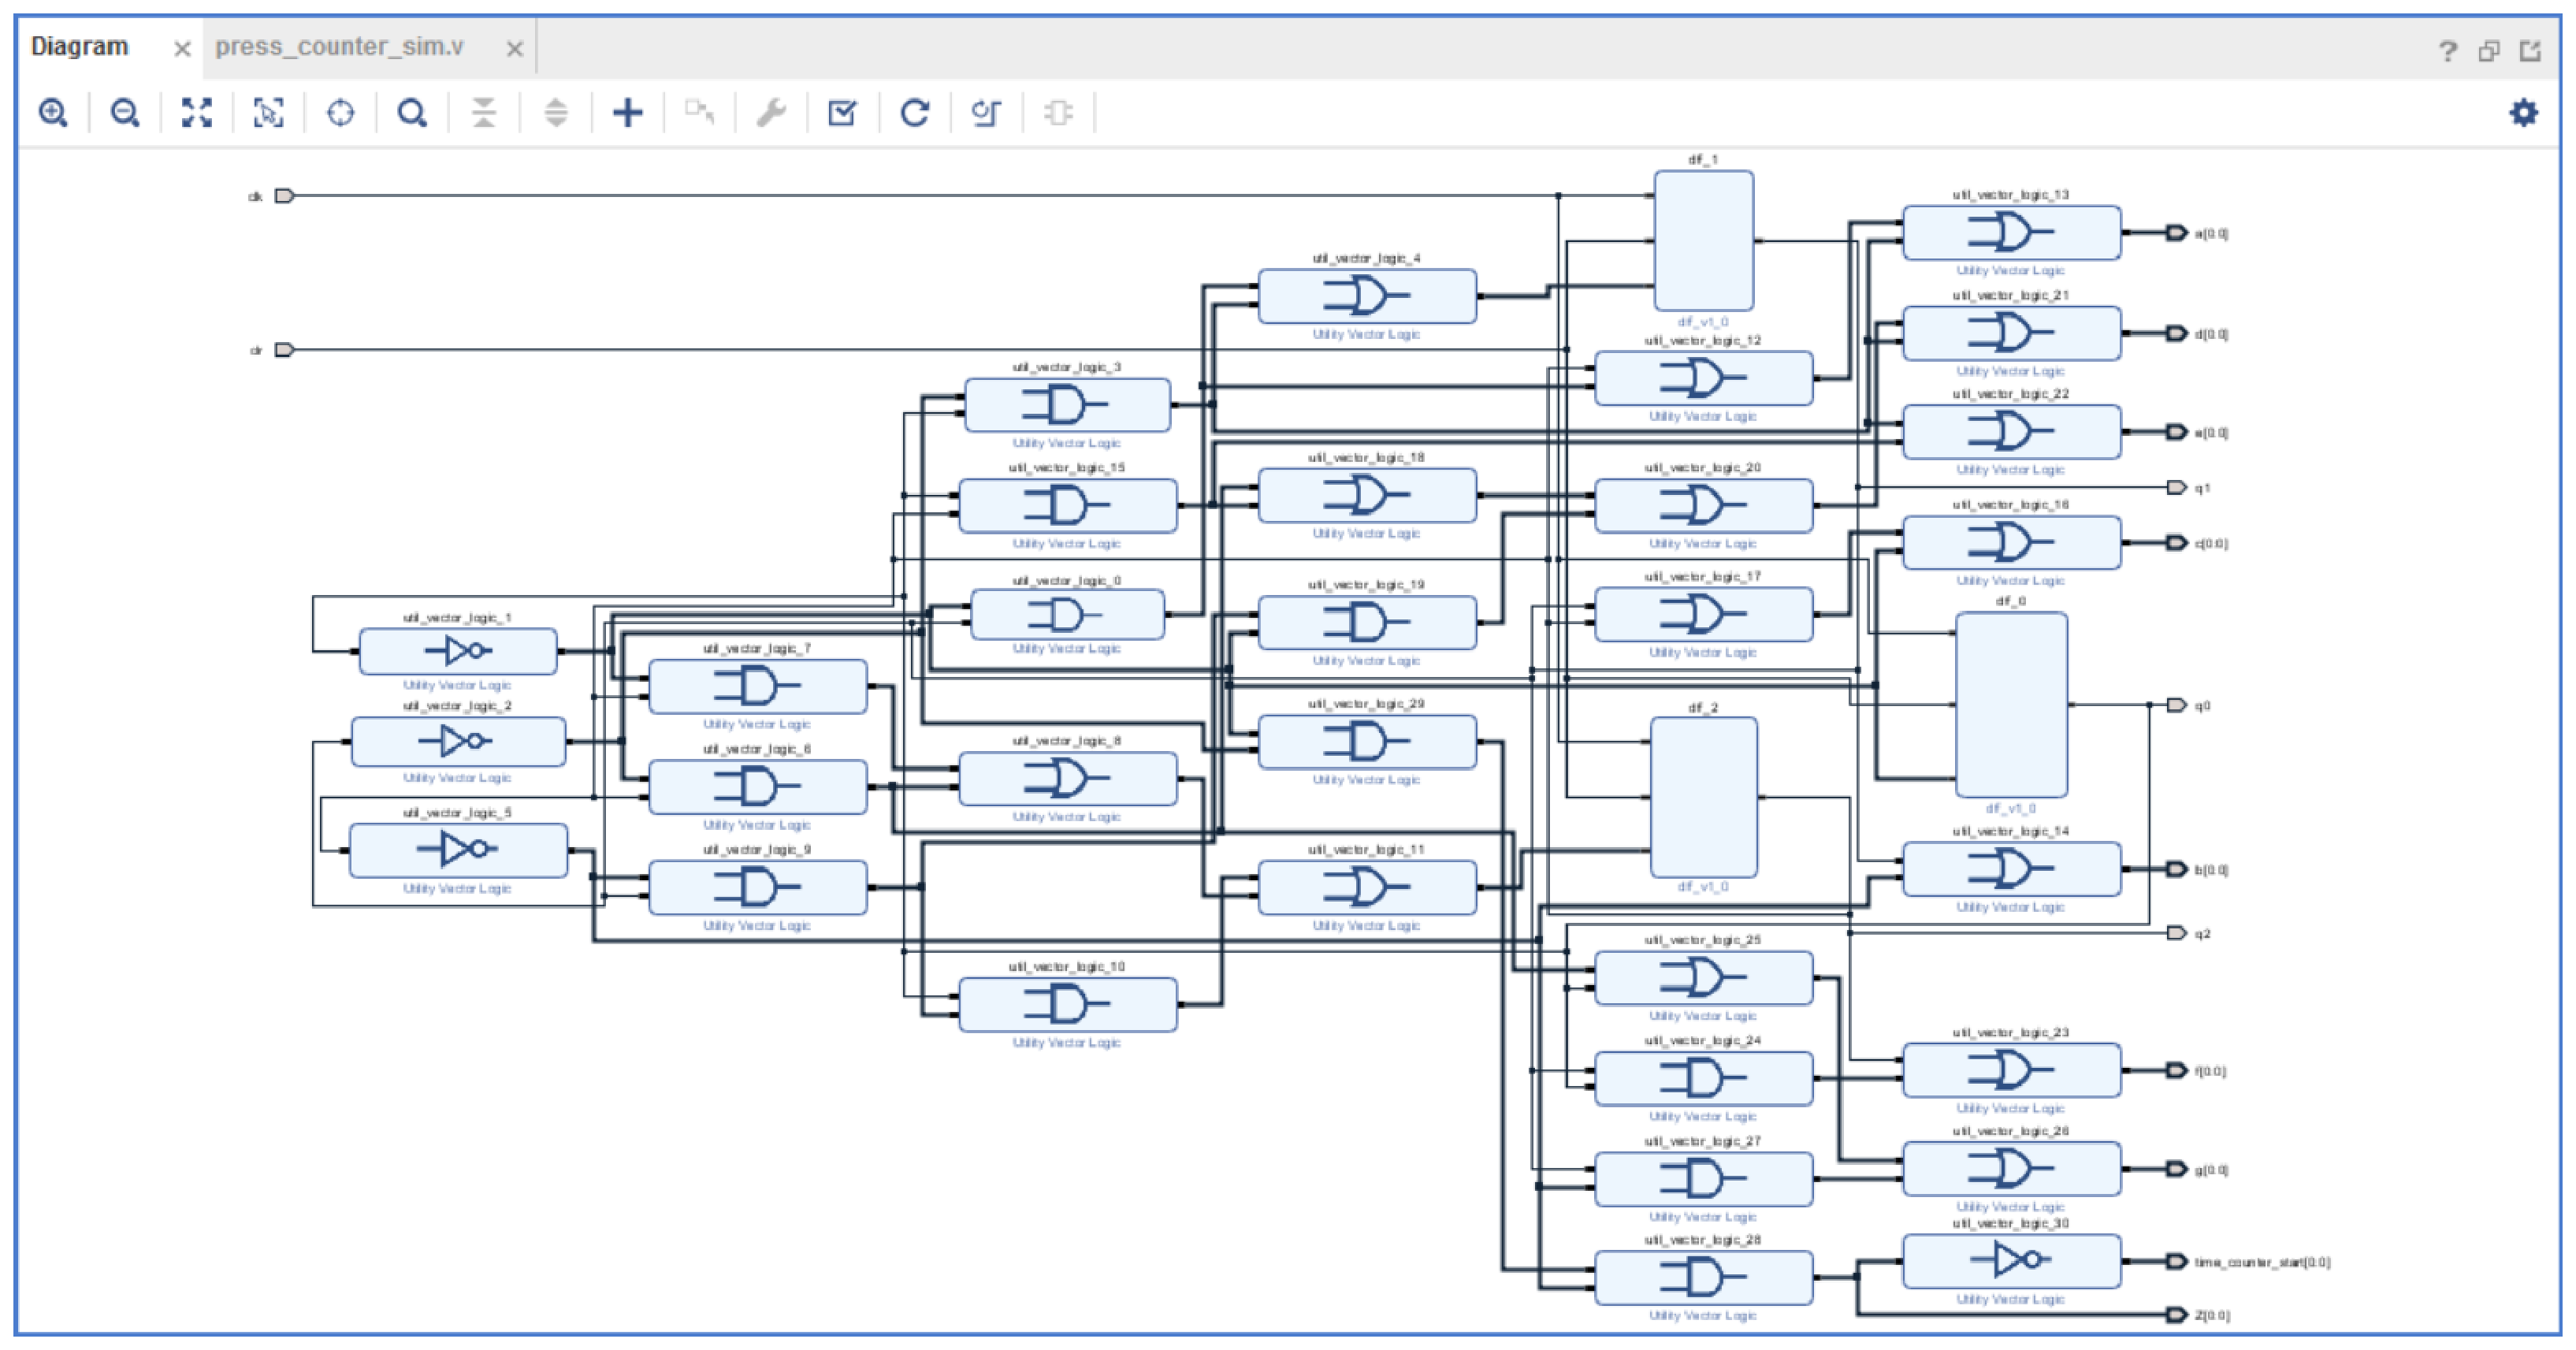
\includegraphics[width =0.9\textwidth]{./images/pic5.eps}
\subsubsection{相关器件}模8计数器,D触发器。

\subsection{显示器}
\subsubsection{选定方案}在计时器和按键计数器上有七段数码管输出端,制作好管脚约束即可显示。
\subsubsection{相关器件}七段数码管。

\section{调试过程}
\subsection{密码表中出现的问题}
\begin{enumerate}
  \item 变量未声明,经检查是变量名写错了,经过简单的修改就又可以正常工作了。

        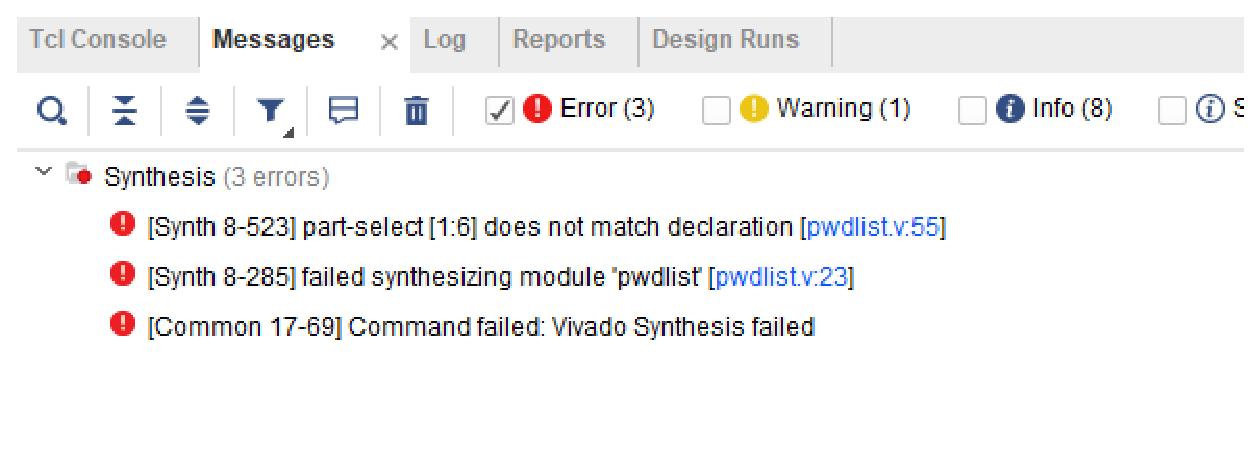
\includegraphics[width=0.9\textwidth]{./images/error0.eps}
  \item 这个错误很棘手,在百度时发现是由于在两个$always$块里修改了同一个$reg$变量,我对修改变量的部分做了综合,使用按键的上升沿进行触发,结果又出现了下面的错误。这也导致其无法自动复位。
        后来经过代码修改,使得在不修改密码时,密码长度计数值自动复位,又成功实现了自动复位。

        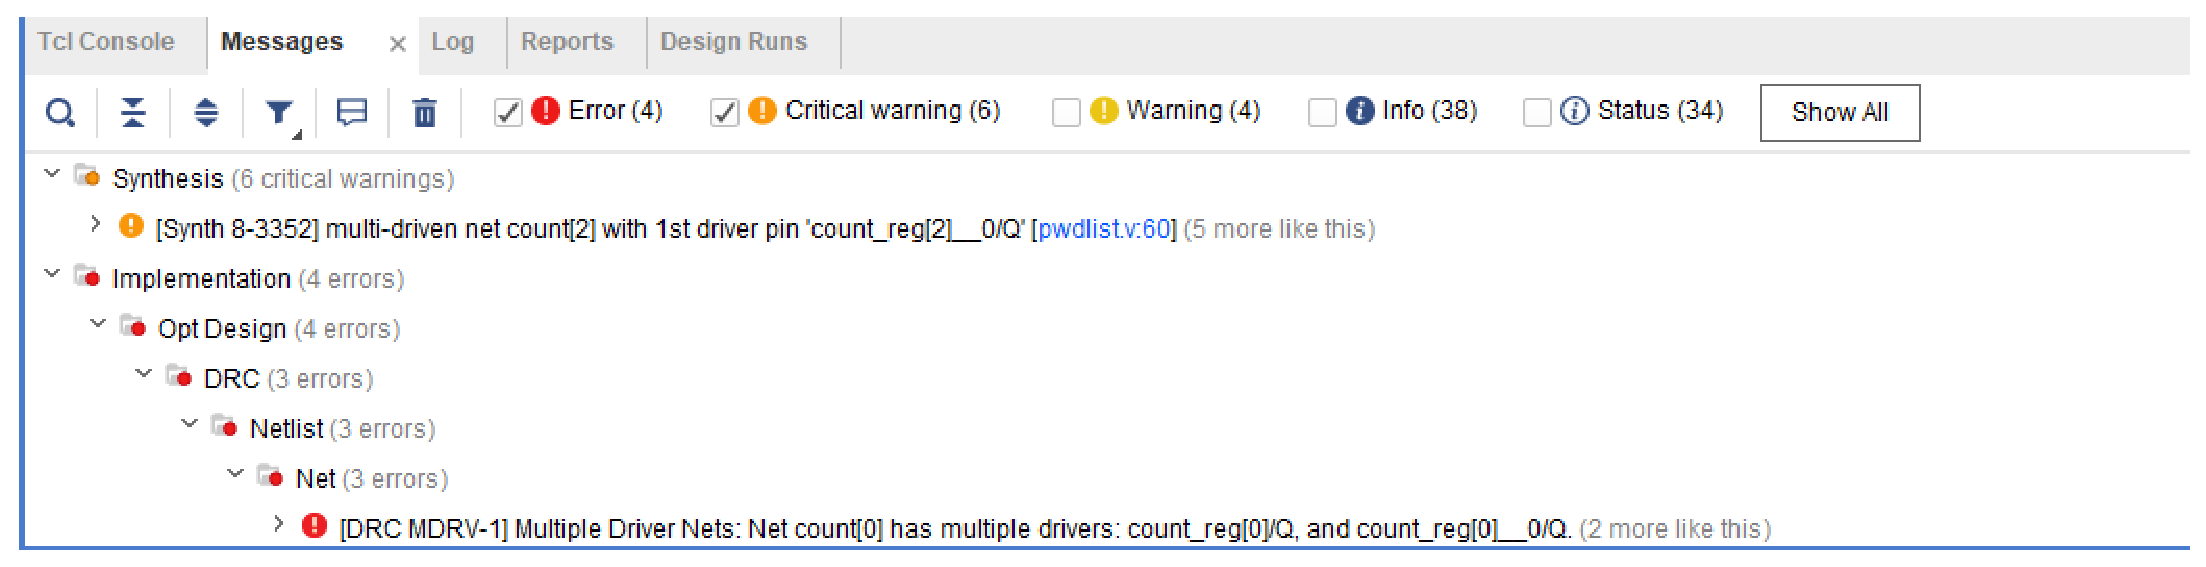
\includegraphics[width=0.9\textwidth]{./images/error4.eps}
  \item 这个错误中提到Pin$R15$不能当作CLK使用,多次研究后,将上升沿触发取消掉,成功。

        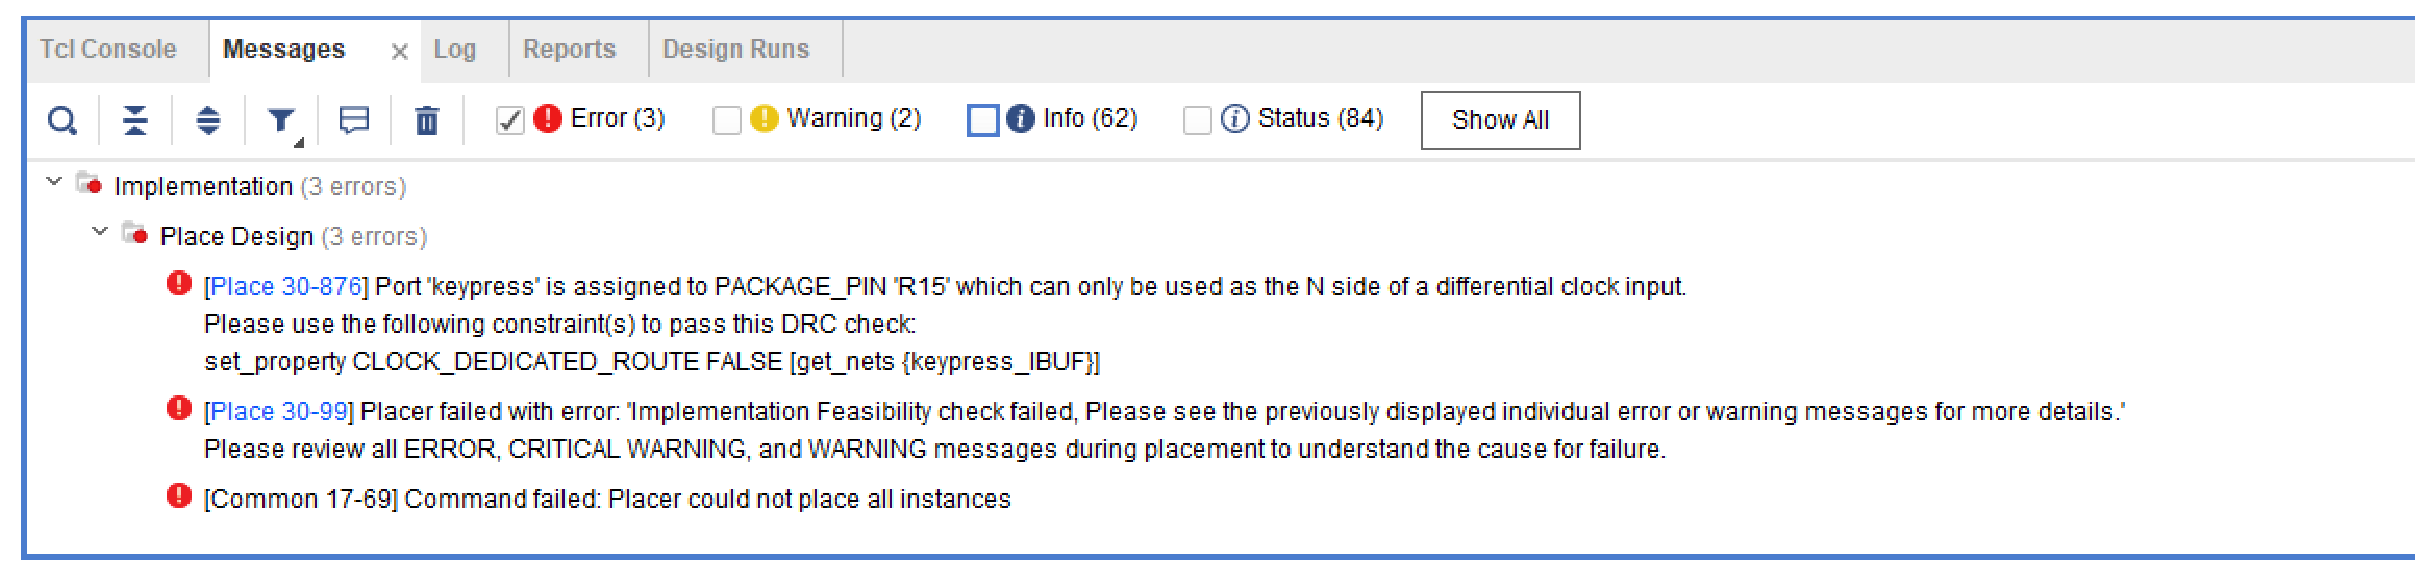
\includegraphics[width=0.9\textwidth]{./images/error5.eps}

  \item 中间调试过程中发现改了一位密码就会改变开锁状态,导致密码修改失败,经过修改,使得密码长度变更发生在密码更改完毕后,解决问题。

  \item 仿真时完全正确,当下载综合到开发板上时,完全不正确。经研究还是密码表的问题,进行大修,重写,测试通过。
\end{enumerate}

\subsection{数码管}
\begin{enumerate}
  \item 数码管会有抖动,查找资料,修改代码,将显示与更改显示值的时间错开,完成数码管消隐。
\end{enumerate}

\subsection{按键处理模块问题}
在按键处理模块中,需要编写延迟器使得按键脉冲能够为密码处理模块提供上升沿时钟信号。写完代码后进行仿真,发现其仿真波形图如下:

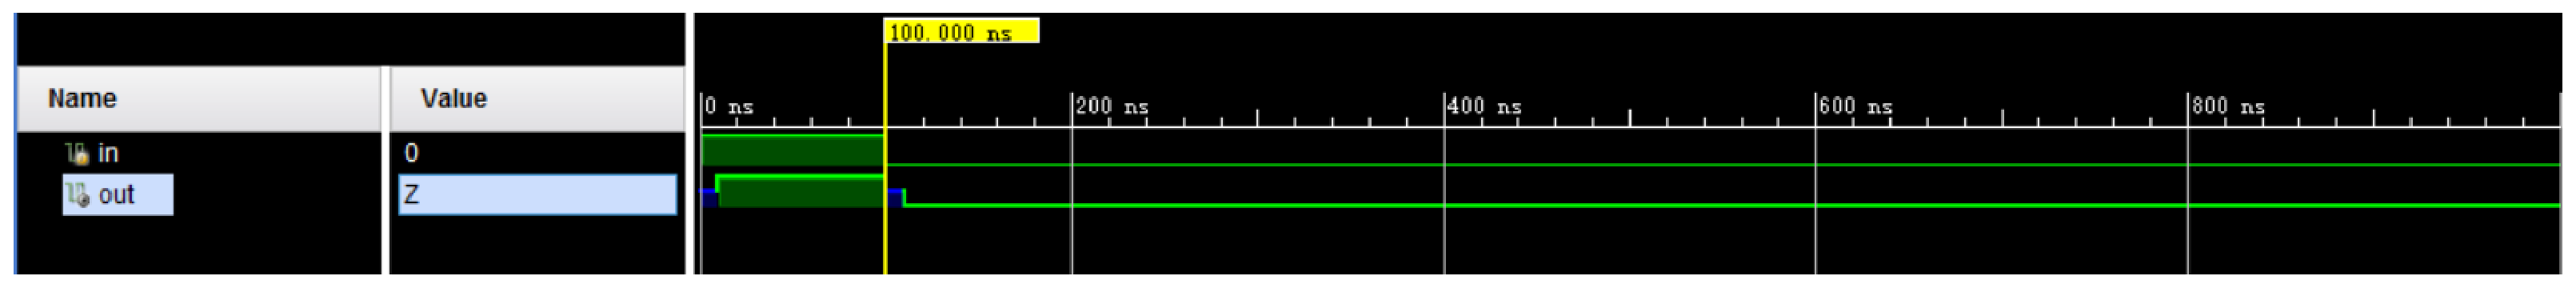
\includegraphics[width=0.9\textwidth]{./images/Lsim1.eps}

在in从高电平转为低电平之后的10ns内,out并没有延续in之前高电平信号,而是变成高阻态,过了10ns才成为低电平状态,延迟器代码出现问题,发现其实只需要在最初始的10ns内为高阻态即可,需要初始化。按照下图
修改之后,波形图为想要的图:

\includegraphics[width=0.4\textwidth]{./images/Lchange1.eps}
\includegraphics[width=0.4\textwidth]{./images/Lchange2.eps}

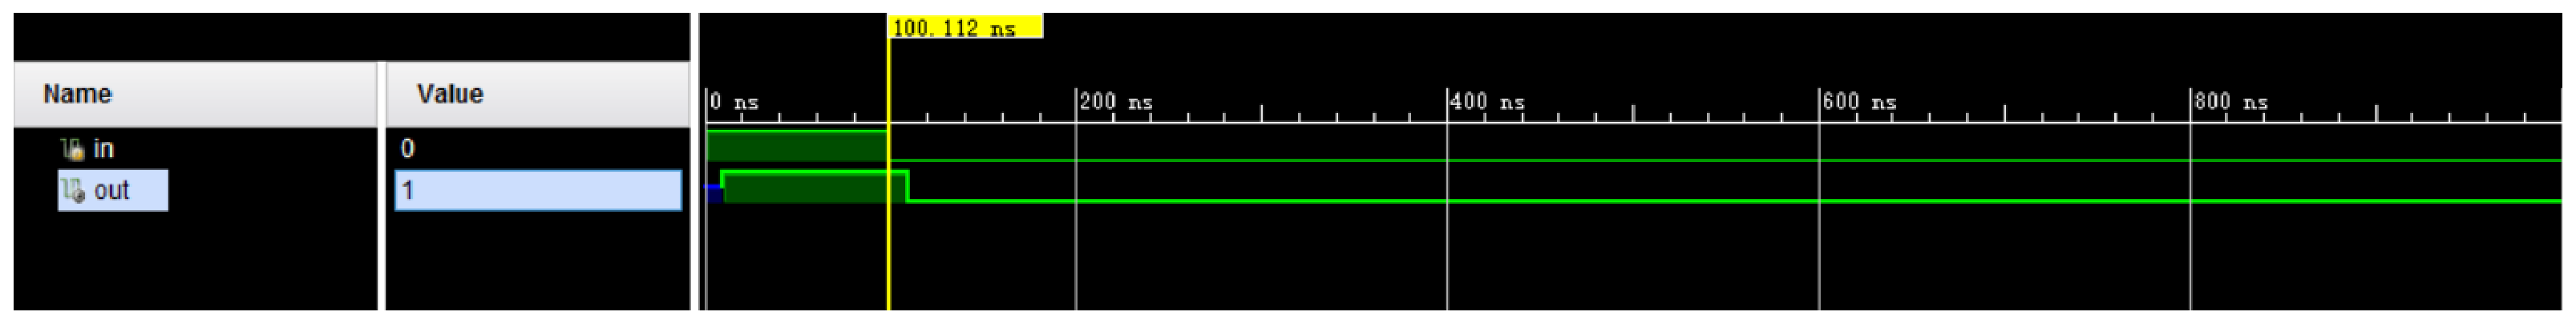
\includegraphics[width=0.9\textwidth]{./images/Lsim2.eps}

在按键计数器模块中,欲用D触发器拼装成一个模8计数器。在编写D触发器时需要异步低效清零端clr,写完代码后进行仿真,却发现自己写的竟然是同步高有效清零了。

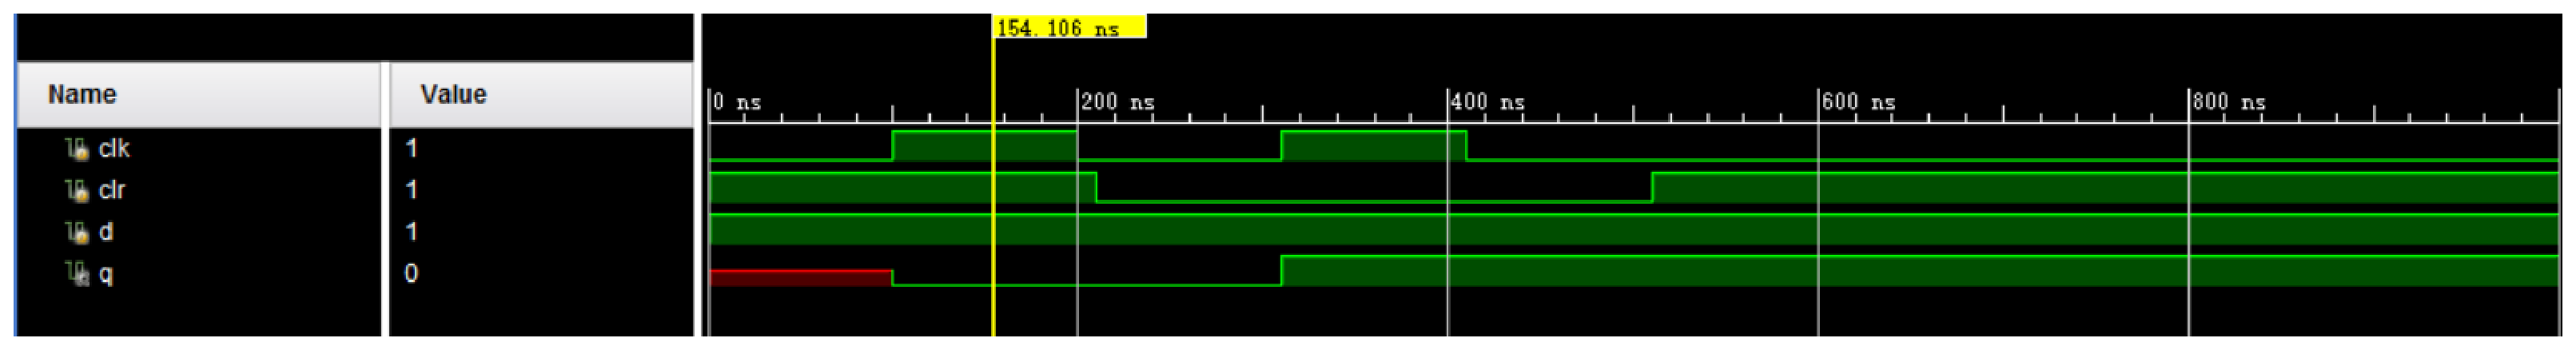
\includegraphics[width=0.9\textwidth]{./images/Lsim3.eps}

经过检查代码,发现在always块的敏感列表除posedge clk外未加clr,导致清零端同步时序。另外再将clr的有效值更改为0即可。

\subsection{计时器模块问题}
在计时器写好代码,仿真、综合、约束管脚之后,发现仿真正确,但是在开发板中调试却得不到结果。起初是不断给时钟上升沿,但就是没有反应,预测时钟端出现不可综合问题。将代码中的“=”改成“<=”后,再次进行仿真、综合,这次发现时钟端有效,但异步清零端无效。最后迫不得已把计时器模块的任务交给了队友冯云龙,得以解决。

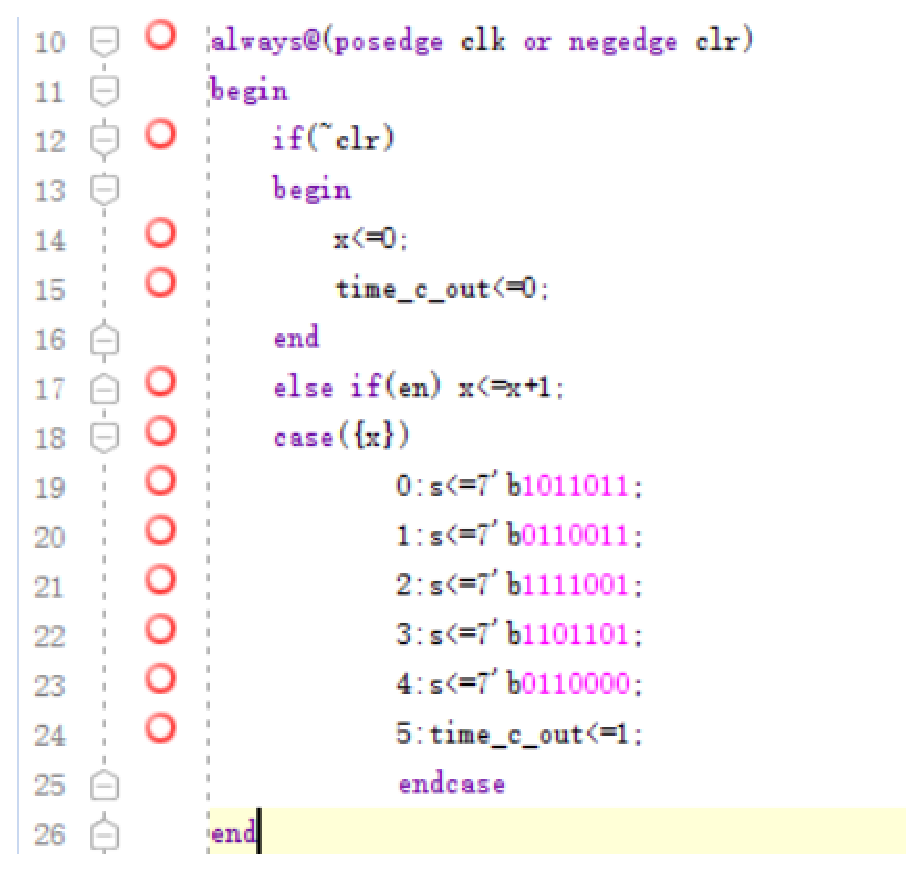
\includegraphics[width=0.9\textwidth]{./images/pic3.eps}

\subsection{组装出现的问题}

在将各组员的工作组装时,拼接block完成之后综合时报错,封装IP时出现差错;再重新封装IP时,出现如图1选项,这时选择如图2选项时,再进行拼接综合后,报错消失。

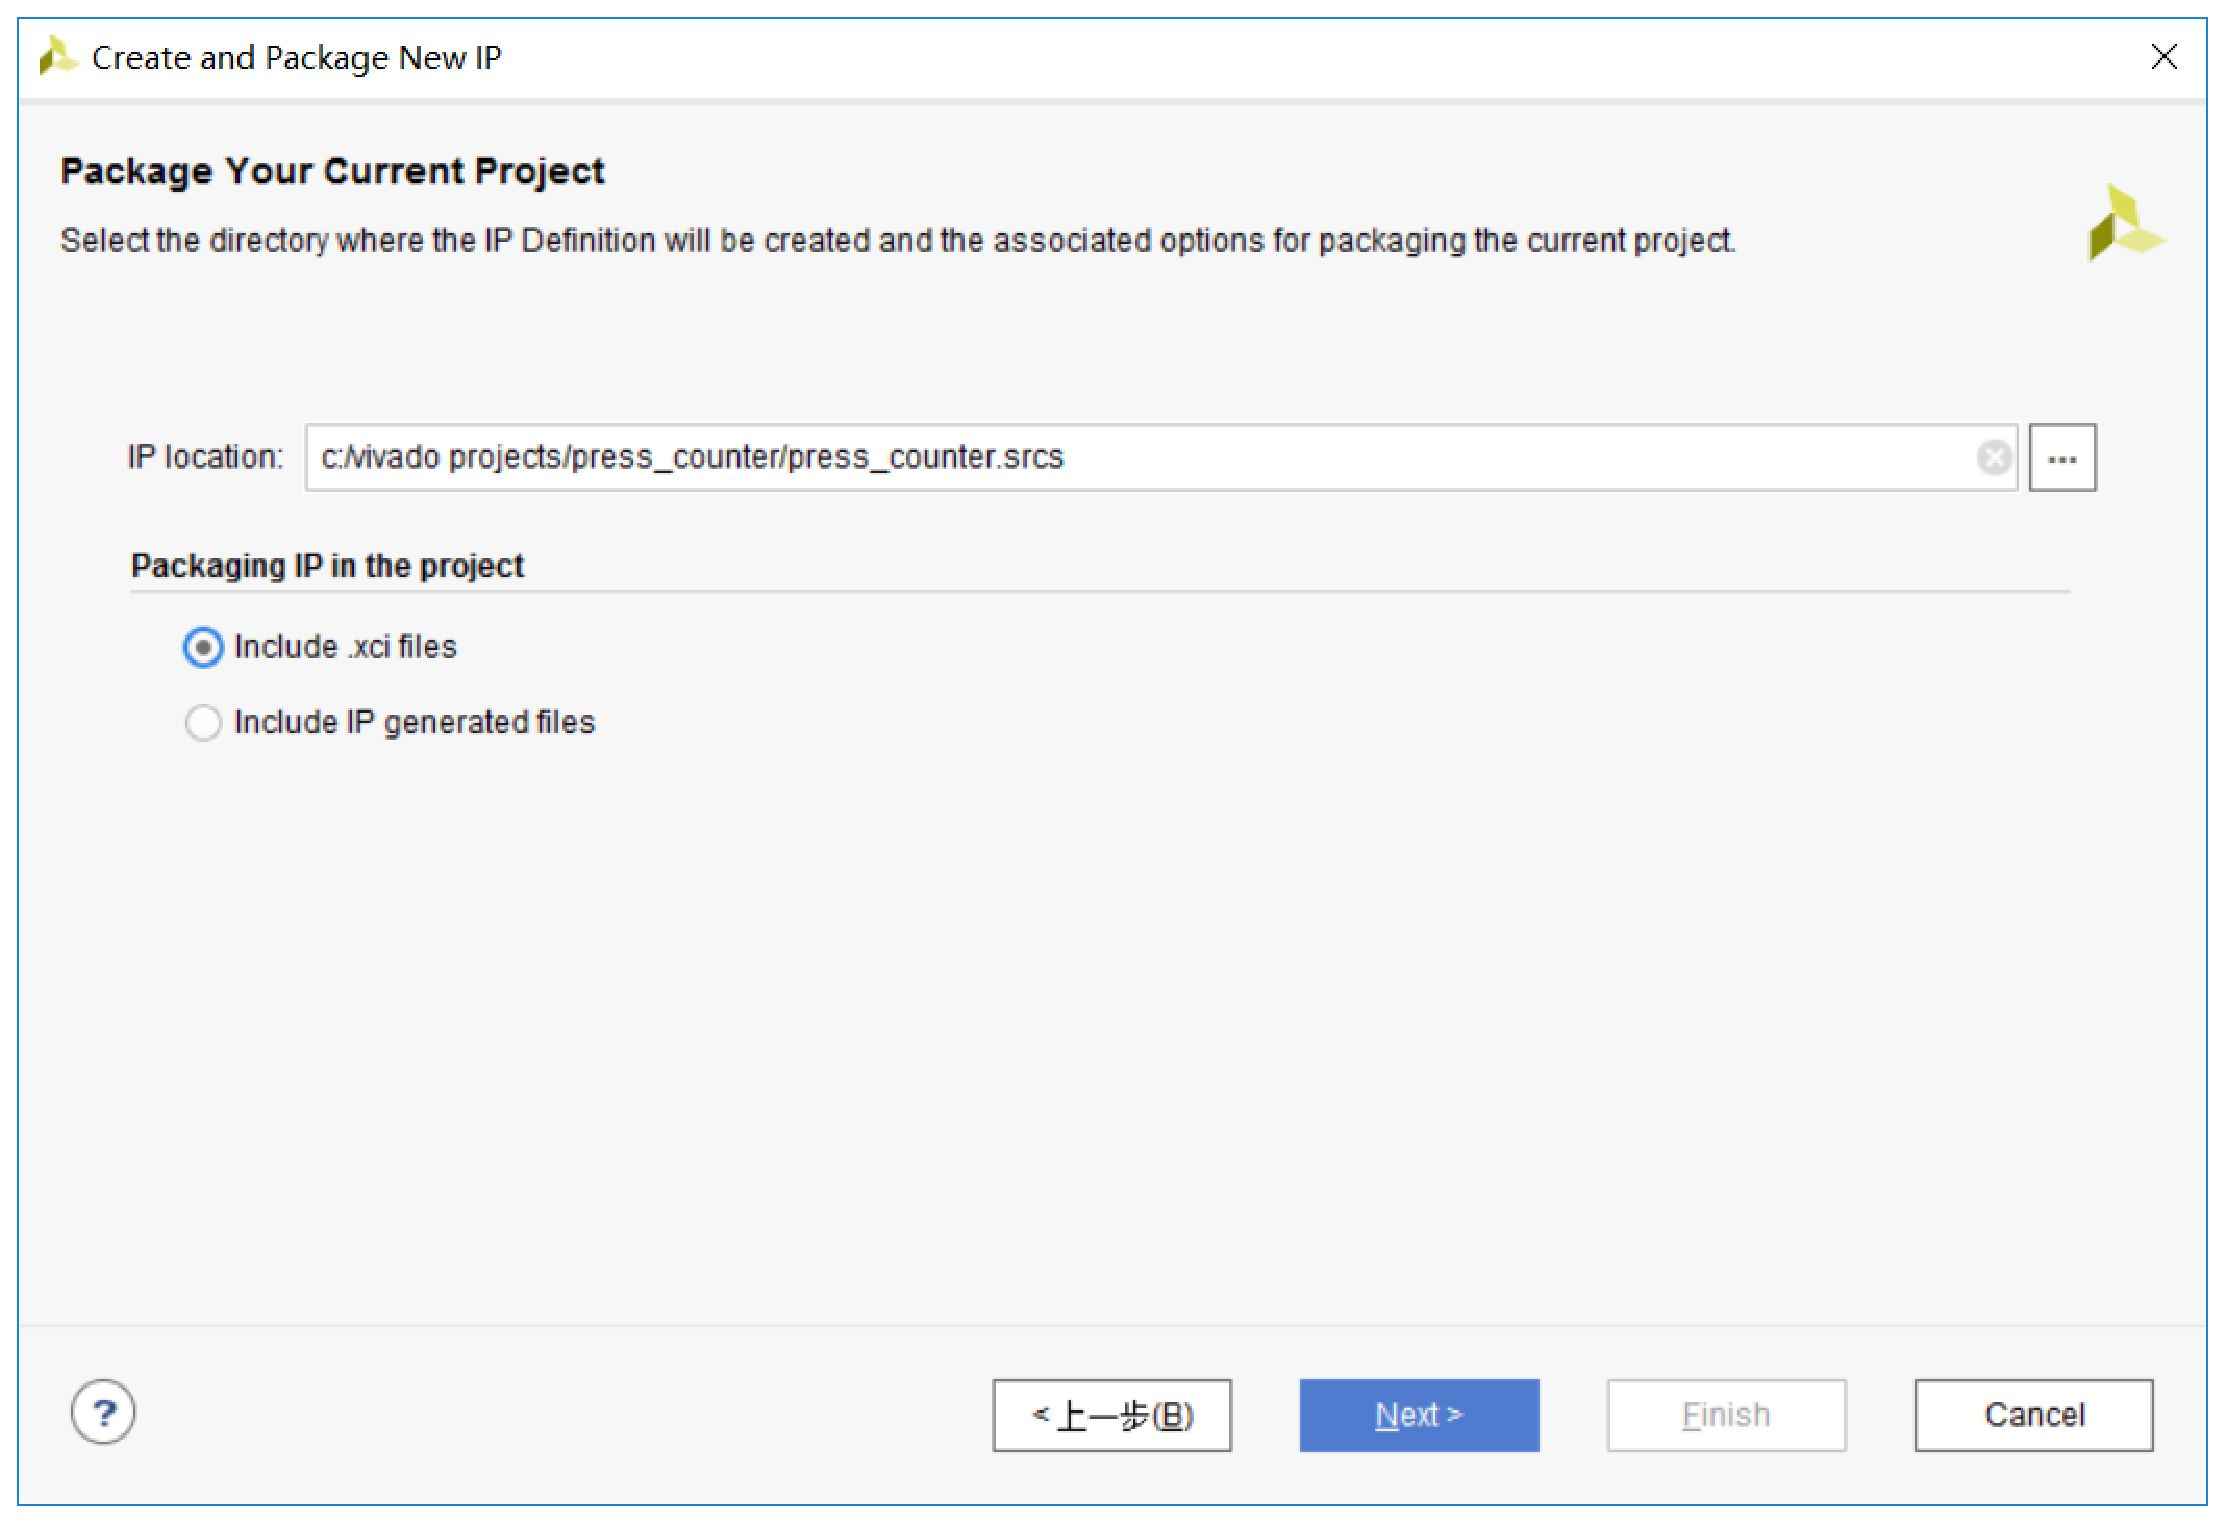
\includegraphics[width=0.9\textwidth]{./images/pic1.eps}

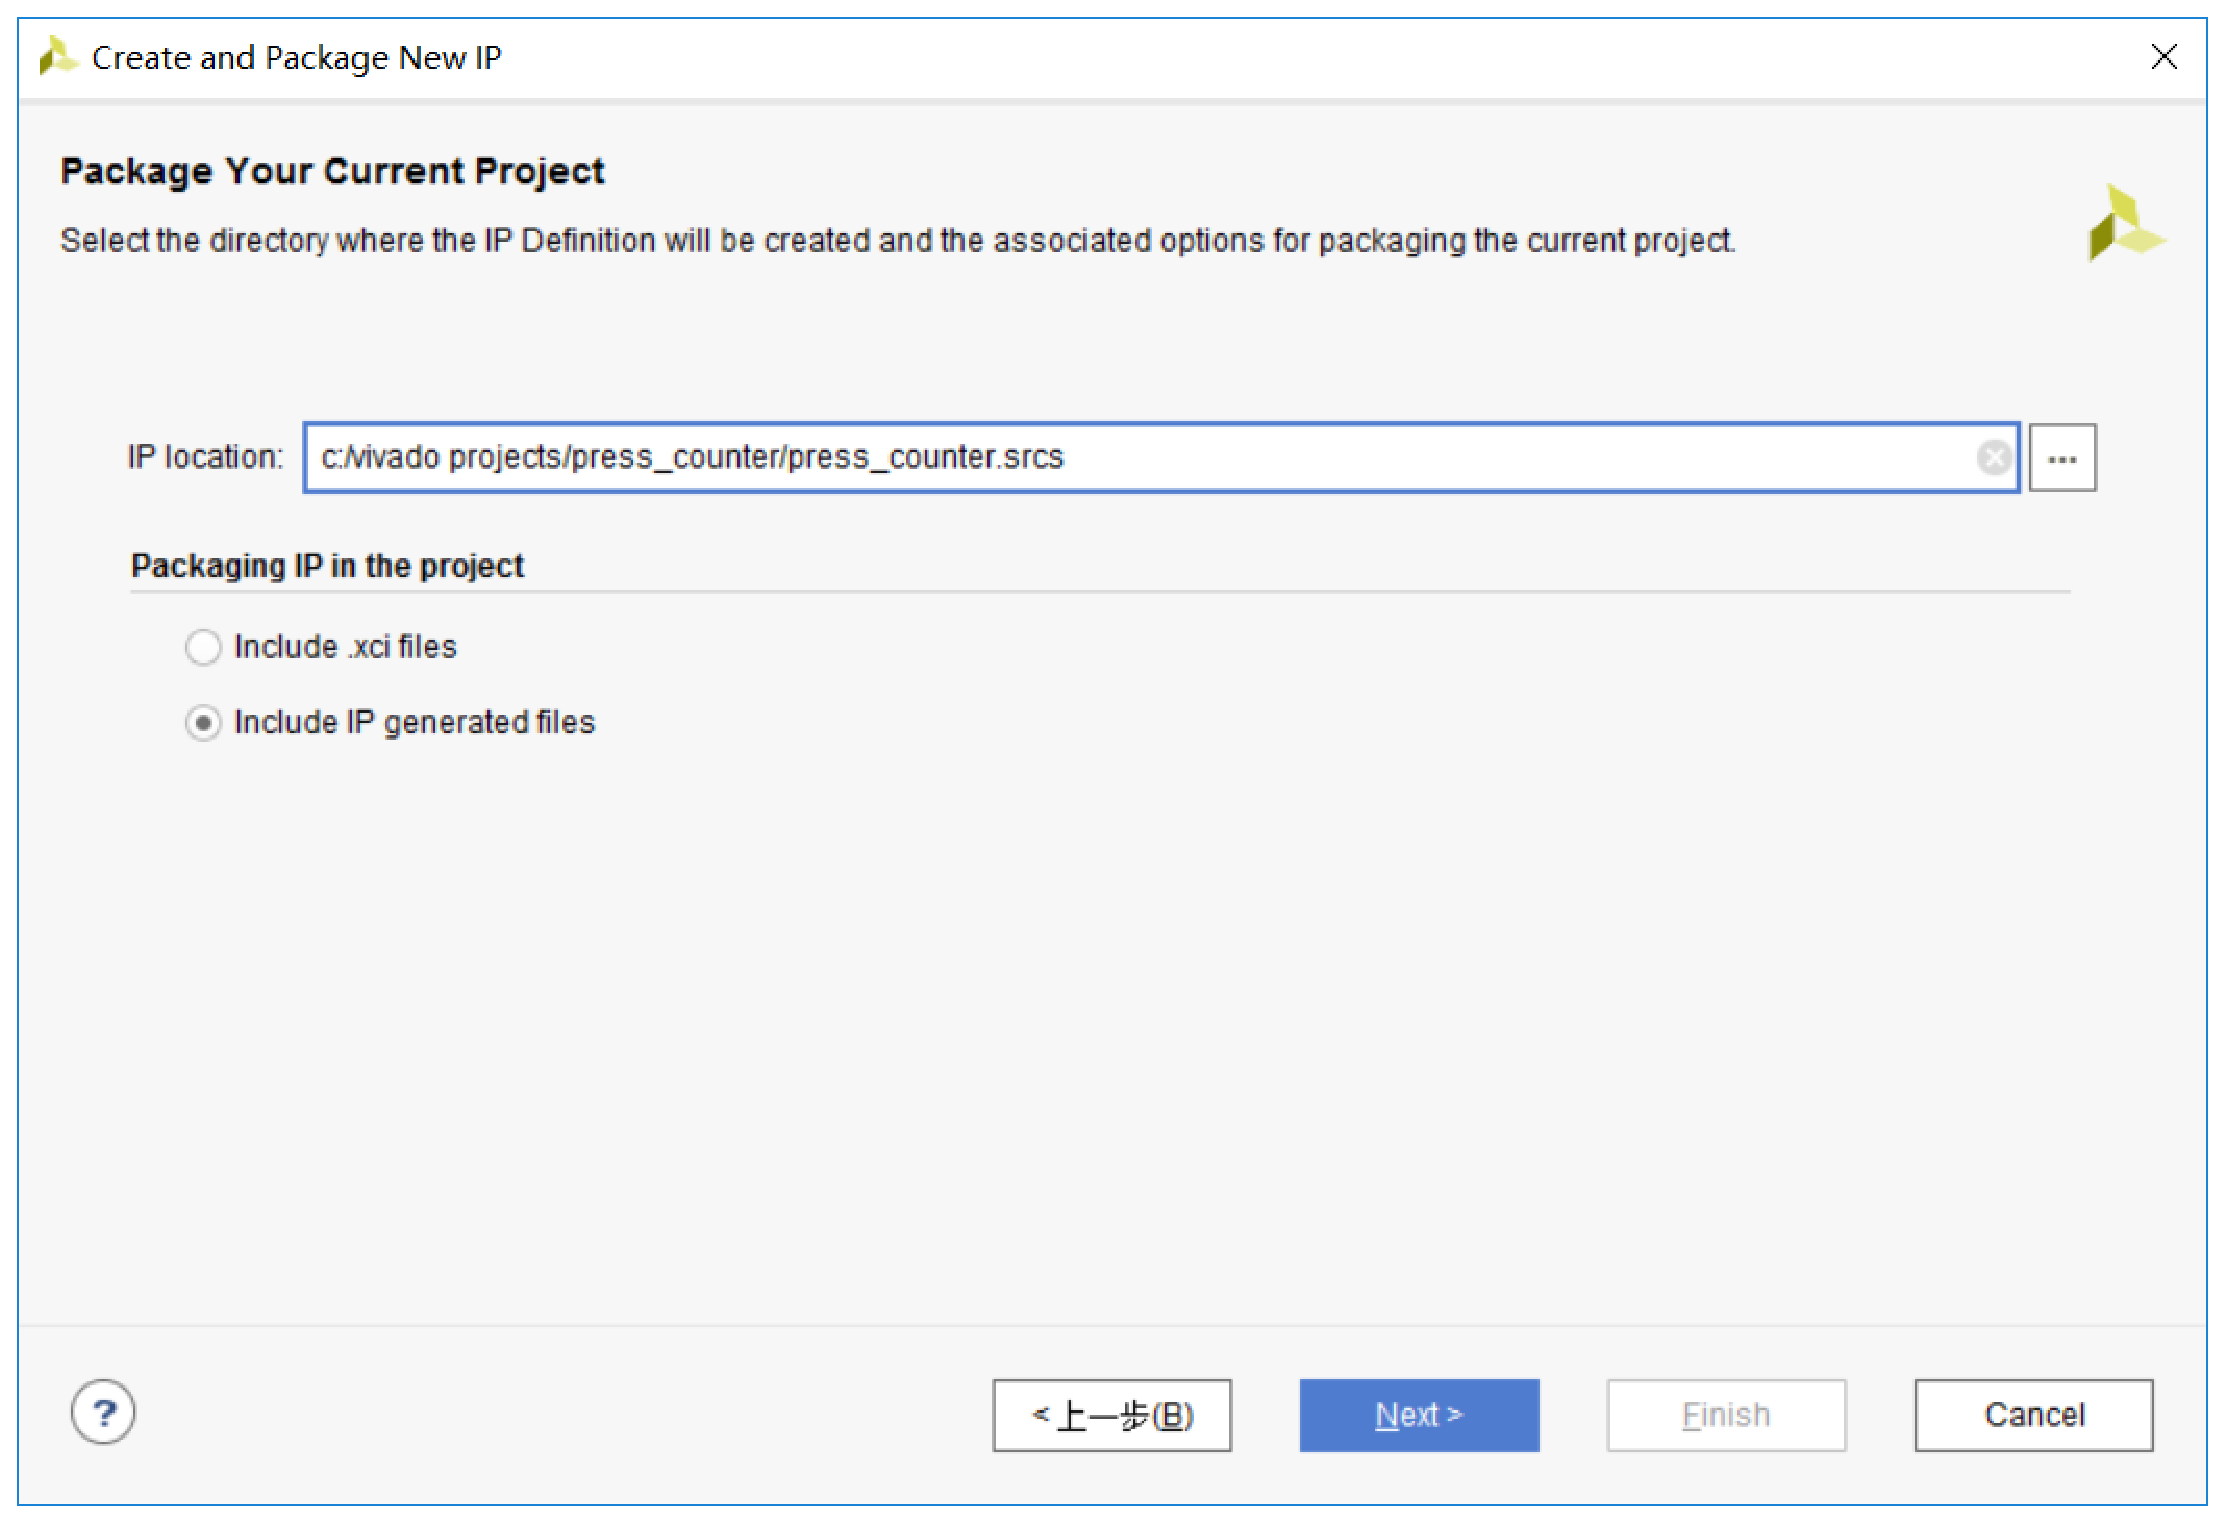
\includegraphics[width=0.9\textwidth]{./images/pic2.eps}

\section{设计结论}
\subsection{项目成果}
通过团队的分工与合作,我们完成了带有三个附加功能的密码锁。可以修改真实密码数值以及位数,并且可以记录当前按键次数,以及输入密码时的时间倒计时进行保障安全。
\subsection{项目团队}
我们的团队一共有两名成员,地位是等同的,分工协作完成了我们的项目。期间我们进行了各种讨论以敲定最终的接口。

\section{设计心得与总结}
\subsection{冯云龙}大作业的设计是曲折的,这次设计让我体会到设计接口的必要性,在设计整个项目的时候,我仿照着计算机界协同工作的一般形式,即先设计接口,再实现功能。
很多时候一个大的工程都不是一个人完成的,而是许许多多的人分工合作完成的,如何协调任务,分配任务是一个很重要的问题。计算机领域的解决方案就是设计接口,这样就隐藏了具体实现,只关注功能的可用性。
每一个模块在设计之初如果就完成了整合,那么每个模块只要按照文档实现,那么实现后一定也能很好的整合。这次的大作业,我们只有两个人,设计的重要性就已经体现出来,更大的工程项目肯定对于设计的要求会更高。
团队的合作,设计是极为重要的。
\subsection{赖昕}在这次大作业的完成过程中,我深切地感受到工程实际实现与理论之间的差距。团队从设计开始,一直到最终的实现,都是坎坷曲折的。最初,我本以为设计出各个模块分好工后就能够一帆风顺地完成作业。然而,实际上我们只花费了半天时间在理论的设计上,在具体操作和调试过程中花费的时间和精力远远大于理论设计上。当设计出具体用什么器件来实现某项功能并写好代码时,vivado会报错;处理好之后写好激励代码进行仿真时,又会发现一系列的错误;在处理好之后进行综合,又会出现不可预知的错误;最后就算历经千辛万苦在vivado上仿真综合全都正确之后,连接到开发板上后又会遇到无效的问题。并且在各组员分工完成进行组装的阶段,也会出现各种各样意想不到的错误。
另外,通过这次大作业,我对vivado更加熟悉了,使用verilog语言编写程序也更加熟练了,对FPGA编程的经验也更加丰富,对各个器件的功能具体实现也有了清晰的认识。此外,我更是接触到了延迟器、分频器等等之前不甚了解的器件的具体实现方法。其中延迟器可以运用移位寄存器来实现,分频器可以运用计数器来进行实现。
最终,整个密码器的实现与整个团队的合作也是密不可分的。正是团队组员之间的合理分工与协作,才能让最终的组装得到满意的结果。也正是这种合理分工,才使得合作有了意义。


\section{参考文献}

\begin{enumerate}
  \item verilog语言实现任意分频 http://blog.csdn.net/ywhfdl/article/details/7641288
  \item verilog 语言关于如何处理一个变量在多个always块里赋值不可综合问题 http://bbs.csdn.net/topics/390752257
  \item 如何解决vivado对时钟端有关问题的报错 http://blog.csdn.net/cnkuaike123/article/details/48403067
  \item FPGA中的延时处理 https://www.mianbaoban.cn/blog/post/64632
  \item 实现信号延时的方法 http://blog.csdn.net/xiangyuqxq/article/details/7255967
  \item verilog入门教程
  \item Tobias Oetiker,Hubert Partl, Irene Hyna and Elisabeth Schlegl,lshort-zh-cn
  \item 单片机数码管显示消隐 http://www.eeworld.com.cn/mcu/article\_2016122332568.html
\end{enumerate}

\newpage
\appendix
\part{附录}
\section{总体器件表及相关器件的功能表、管脚分布}
\subsection{密码长度计数器}
\begin{figure}[htb]
  \begin{minipage}[b]{0.5\textwidth}
    \centering
    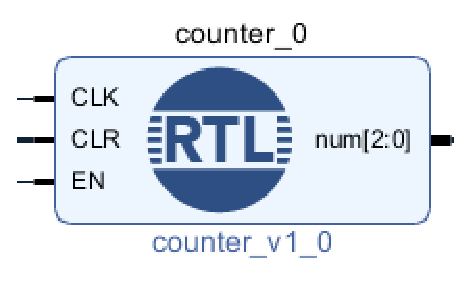
\includegraphics[width = \textwidth]{./images/counter.eps}
    \caption{密码长度计数器}
    \label{fig:by:table}
  \end{minipage}%
  \begin{minipage}[b]{0.5\textwidth}
    \centering
    \begin{tabular}{|c|c|} \hline
      管脚名 & 功能                                            \\ \hline\hline
      CLK       &   上升沿触发计数      \\
      CLR       & 异步清零端                     \\
      EN        & 使能端                             \\
      num       & 当前密码输对的个数    \\ \hline
    \end{tabular}
    \caption{功能表}
    \label{table:by:fig}
  \end{minipage}
\end{figure}

\subsection{密码处理}
\begin{figure}[htb]
  \begin{minipage}[b]{0.5\textwidth}
    \centering
    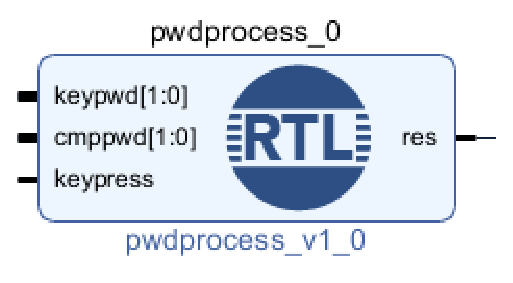
\includegraphics[width = \textwidth]{./images/pwdprocess.eps}
    \caption{密码处理}
    \label{fig:by:table}
  \end{minipage}%
  \begin{minipage}[b]{0.5\textwidth}
    \centering
    \begin{tabular}{|c|c|} \hline
      管脚名 & 功能 \\ \hline\hline
      keypwd    &   按键输入密码 \\
      cmppwd    & 正确密码输入端 \\
      keypress  & 按键脉冲,有按键 \\
      res       &  比对结果 \\ \hline
    \end{tabular}
    \caption{功能表}
    \label{table:by:fig}
  \end{minipage}
\end{figure}

\subsection{开锁控制器}
\begin{figure}[htb]
  \begin{minipage}[b]{0.5\textwidth}
    \centering
    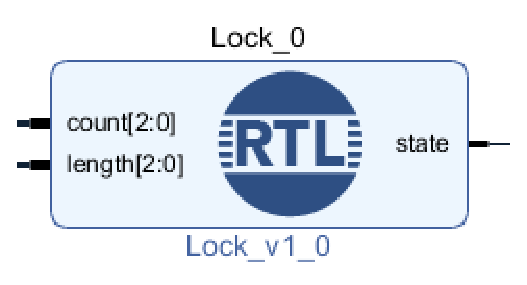
\includegraphics[width = \textwidth]{./images/Lock.eps}
    \caption{开锁控制器}
    \label{fig:by:table}
  \end{minipage}%
  \begin{minipage}[b]{0.5\textwidth}
    \centering
    \begin{tabular}{|c|c|} \hline
      管脚名 & 功能 \\ \hline\hline
      count     &   当前输入正确密码的位数 \\
      length    &   正确密码总长度 \\
      state     & 当前开锁状态 \\ \hline
    \end{tabular}
    \caption{功能表}
    \label{table:by:fig}
  \end{minipage}
\end{figure}

\subsection{密码表}
\begin{figure}[htb]
  \begin{minipage}[b]{0.5\textwidth}
    \centering
    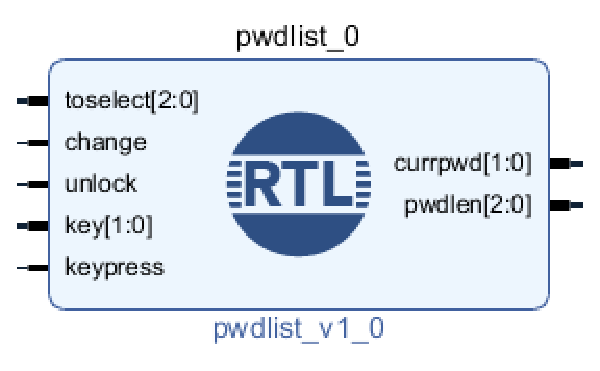
\includegraphics[width = \textwidth]{./images/pwdlist.eps}
    \caption{密码表}
    \label{fig:by:table}
  \end{minipage}%
  \begin{minipage}[b]{0.5\textwidth}
    \centering
    \begin{tabular}{|c|c|} \hline
      管脚名 & 功能 \\ \hline\hline
      toseclect     &   选择的密码 \\
      change        & 是否修改密码 \\
      unlock        & 是否已开锁 \\
      key           & 按键值 \\
      keypress      & 按键脉冲 \\
      currpwd       & 当前正确密码\\
      pwdlen        & 密码长度 \\ \hline
    \end{tabular}
    \caption{功能表}
    \label{table:by:fig}
  \end{minipage}
\end{figure}

\subsection{核心综合}
\begin{figure}[htb]
  \begin{minipage}[b]{0.5\textwidth}
    \centering
    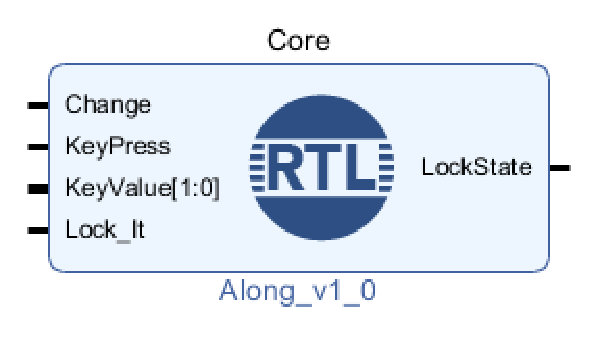
\includegraphics[width = \textwidth]{./images/AlongCore.eps}
    \caption{核心综合}
    \label{fig:by:table}
  \end{minipage}%
  \begin{minipage}[b]{0.5\textwidth}
    \centering
    \begin{tabular}{|c|c|} \hline
      管脚名 & 功能 \\ \hline\hline
      Change        &   修改密码使能                       \\
      KeyPress      &   给按键计数器的按键脉冲  \\
      KeyValue      &   按键值                                    \\
      LockIt       &   上锁信号                                \\
      LockState     &   开锁状态                                \\ \hline
    \end{tabular}
    \caption{功能表}
    \label{table:by:fig}
  \end{minipage}
\end{figure}


\subsection{按键部分}

\begin{figure}[htb]
  \begin{minipage}[b]{0.5\textwidth}
    \centering
    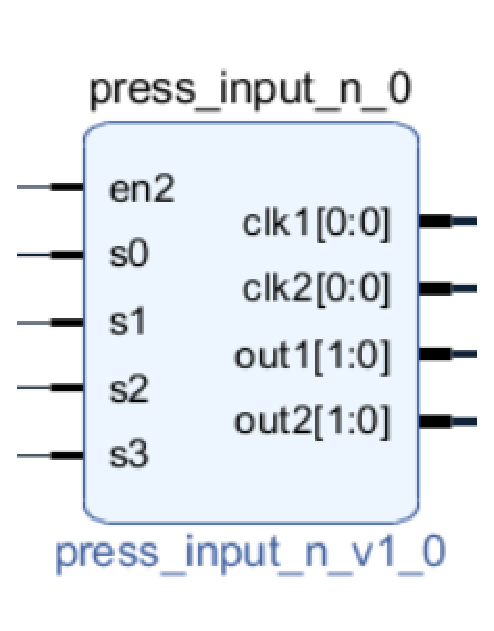
\includegraphics[height= 5cm]{./images/p2.eps}
    \caption{按键部分}
    \label{fig:by:table}
  \end{minipage}%
  \begin{minipage}[b]{0.5\textwidth}
    \centering
    \begin{tabular}{|c|c|} \hline
      管脚名 & 功能 \\ \hline\hline
      clk1     &   脉冲信号(给密码处理)\\
      clk2     & 按键脉冲(给按键计数器) \\
      en2      & 修改密码输出使能 \\
      out1     & 输入密码输出(给密码处理) \\
      out2     & 修改密码输出 \\
      s0~s3    & 按键输入 \\ \hline
    \end{tabular}
    \caption{功能表}
    \label{table:by:fig}
  \end{minipage}
\end{figure}

\newpage
\subsection{按键计数器部分}

\begin{figure}[htb]
  \begin{minipage}[b]{0.5\textwidth}
    \centering
    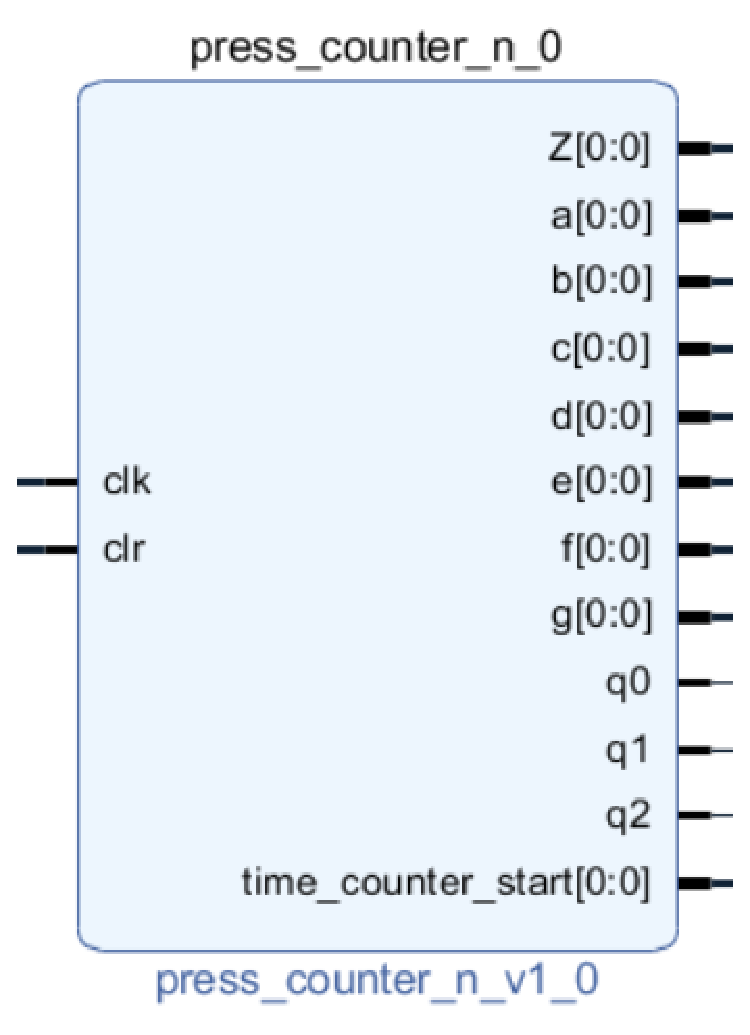
\includegraphics[height= 5cm]{./images/p1.eps}
    \caption{按键计数器部分}
    \label{fig:by:table}
  \end{minipage}%
  \begin{minipage}[b]{0.5\textwidth}
    \centering
    \begin{tabular}{|c|c|} \hline
      管脚名 & 功能 \\ \hline\hline
      clk      &  按键脉冲(来自按键处理)\\
      clr      & 异步清零端(低有效) \\
      Z        & 满八进一的输出(给计数器提供的复位信号) \\
      a~g      & 七段数码管输出 \\
      q0~q2    & 当前计数的三位2进制表示数 \\
      start    & 开始计数信号(给计时器提供) \\ \hline
    \end{tabular}
    \caption{功能表}
    \label{table:by:fig}
  \end{minipage}
\end{figure}


\section{总体设计图}

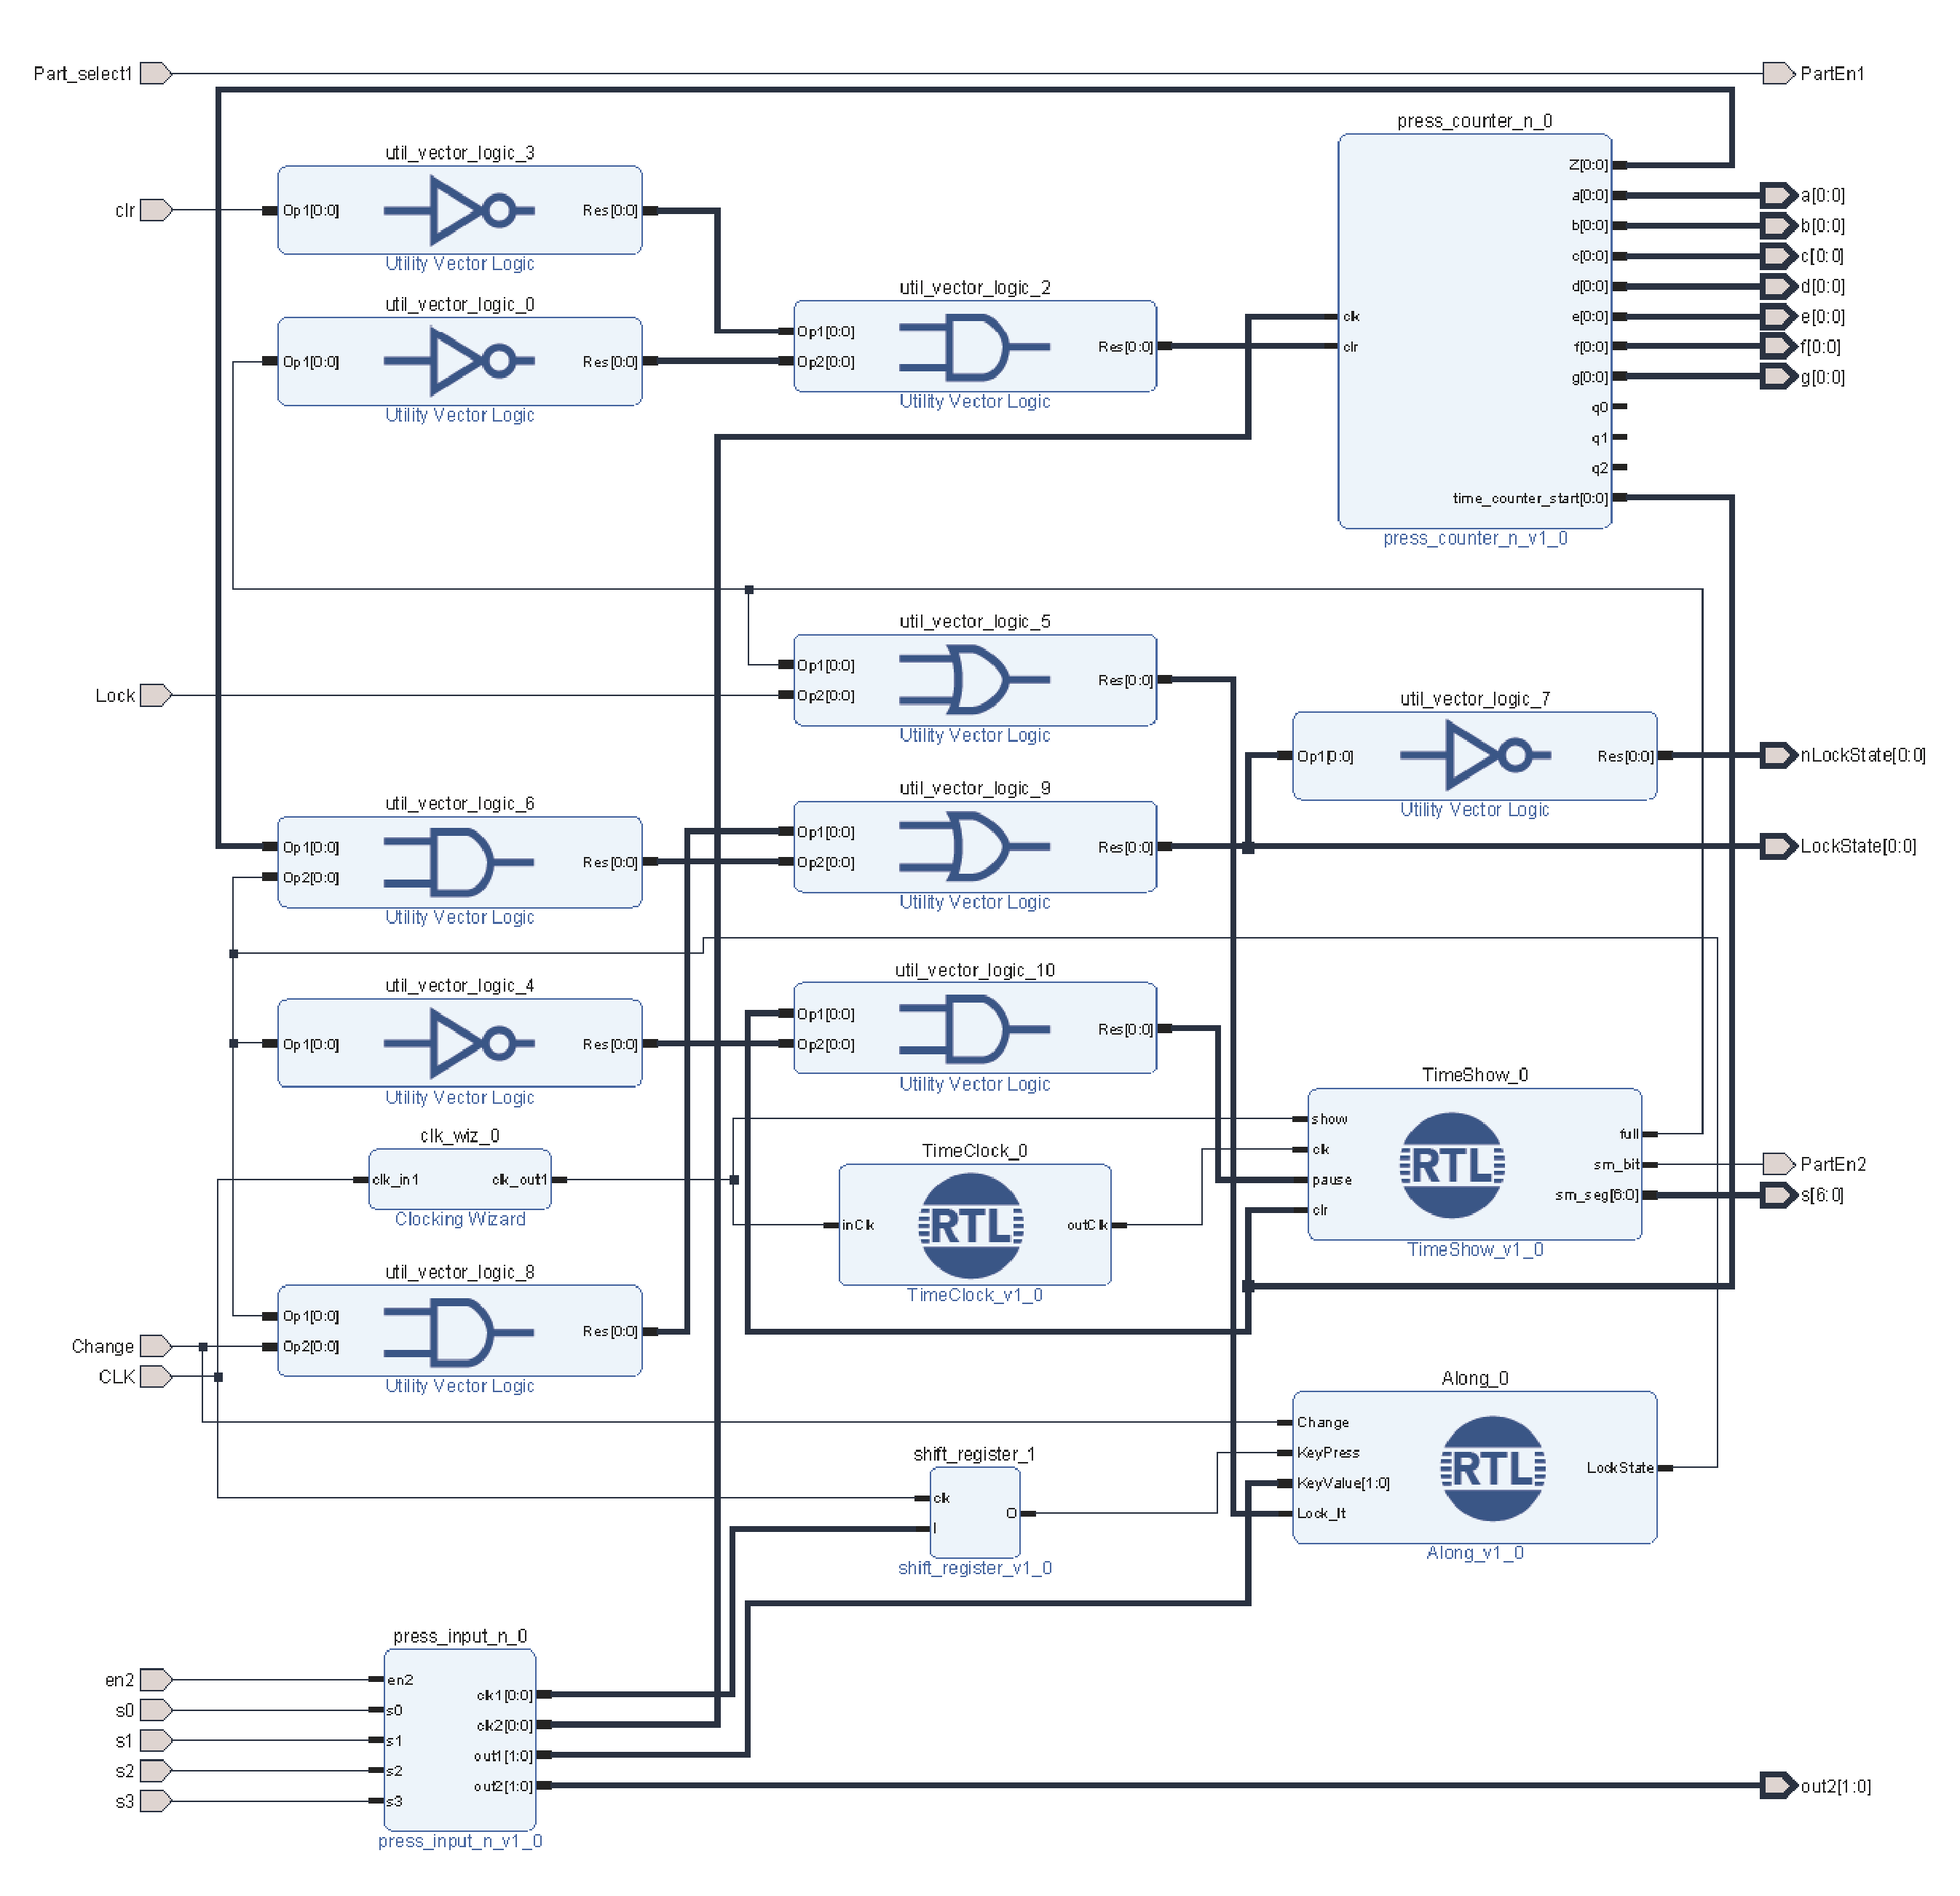
\includegraphics[width=0.9\textwidth]{./images/electric_lock.eps}

\section{仿真结果}
\subsection{A部分仿真}
\paragraph{仿真激励代码}
\begin{lstlisting}[language={verilog}]
module Test();
reg Press;
reg [1:0]key_in;
wire out;

pwdprocess u0(key_in,3,Press,out);  //预设密码为3

initial begin
Press=0;
key_in=0;
end

always #2 Press=~Press;
always #4 key_in = key_in +1;

endmodule
\end{lstlisting}
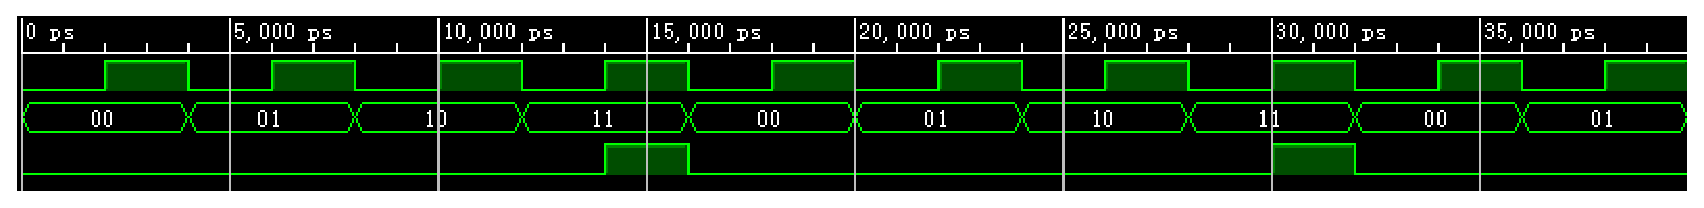
\includegraphics[width=0.9\textwidth]{./images/sim1.eps}

预设的密码为3,经过仿真,输入为3是才能获得正确的脉冲,否则无效。
\paragraph{开锁控制器}
\begin{lstlisting}[language={verilog}]
module Test();
reg [2:0]count;
reg [2:0]length;
wire state;

Lock u0(count,length,state);

initial begin
count=0;
length=5;
end

always #2 count=count+1;

endmodule
\end{lstlisting}
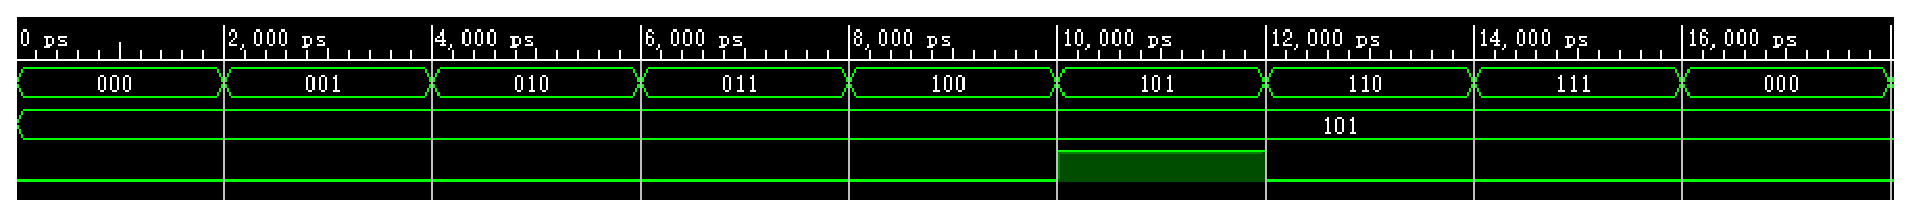
\includegraphics[width=0.9\textwidth]{./images/sim2.eps}

预设的密码长度为5,经过仿真,输入的正确密码为5是才能获得开锁状态。

\paragraph{密码计数器}
\begin{lstlisting}[language={verilog}]
module Test();
reg clk;
reg clr;
wire [2:0]state;

counter u0(clk,clr,state);

initial begin
clk=0;
clr=0;
end

always #2 clk=~clk;

always begin
#35 clr = 1;
#4 clr = 0;end

endmodule
\end{lstlisting}
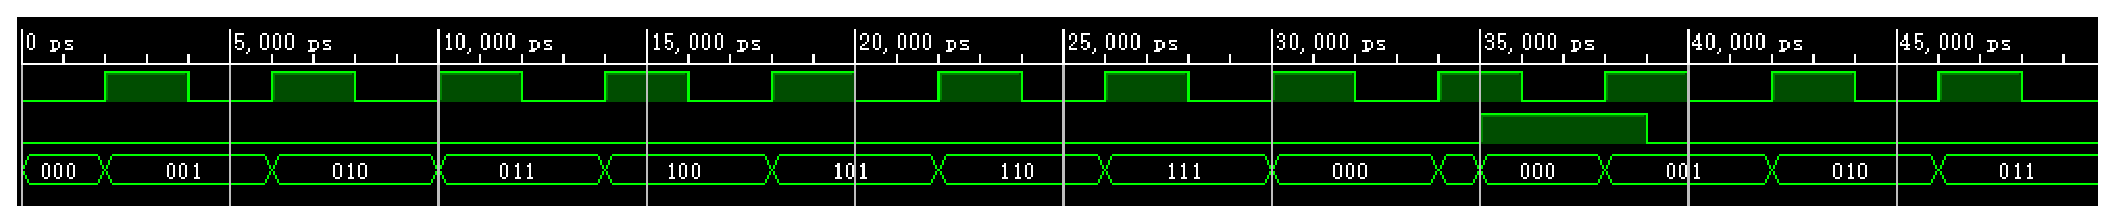
\includegraphics[width=0.9\textwidth]{./images/sim3.eps}

获得一次clk记一次数,上升沿有效,异步清零。

\paragraph{密码表}
\begin{lstlisting}[language={verilog}]
module Test();
reg [2:0]select;        //选择下一位的正确密码
wire [1:0]beSelect;     //被选择出来的密码
wire [2:0]len;          //存储的密码长度

reg change;             //是否修改密码
reg unlock;             //当前开锁状态
reg [1:0]key;           //修改密码所给的值
reg keypress;           //按键脉冲

pwdlist u0(select,beSelect,len,change,unlock,key,keypress);

initial begin
select = 0;
change = 1;
unlock = 1;
key = 0;
keypress = 0;
end

always #2 select=select+1;
always begin
#2 keypress = ~keypress;
key = key + 1;
end

endmodule
\end{lstlisting}
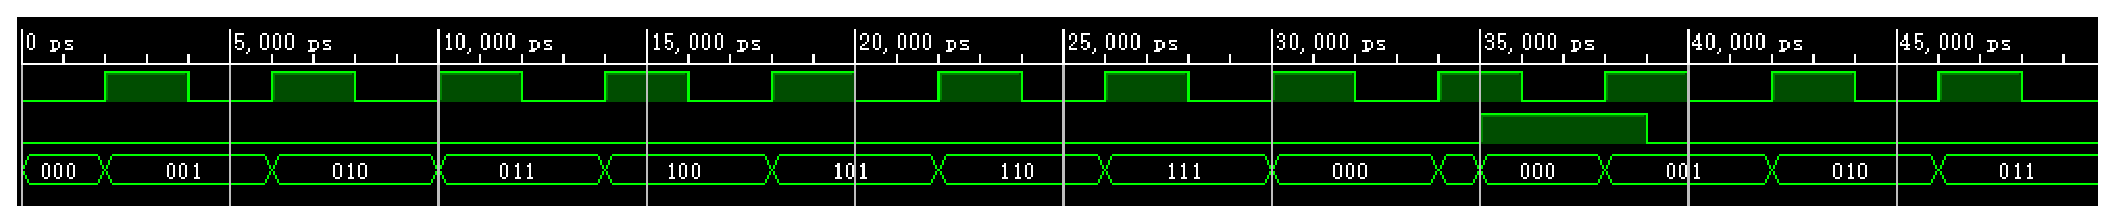
\includegraphics[width=0.9\textwidth]{./images/sim3.eps}

可以修改密码,最多7位,初始密码为0000。

\paragraph{核心功能仿真}
\begin{lstlisting}[language={verilog}]
module Test();
wire LockState;
reg Change;             //是否修改密码
reg Lock_It;             //当前开锁状态
reg [1:0]KeyValue;           //修改密码所给的值
reg Keypress;           //按键脉冲

Along u0(
    Change,
    Keypress,
    KeyValue,
    Lock_It,
    LockState
    );
initial begin
    Change=0;
    Lock_It=0;
    KeyValue=0;
    Keypress=0;
    //上锁
    #2 Lock_It = 1;
    #2 Lock_It = 0;
    //开锁
    #2 Keypress = ~Keypress;
    #2 Keypress = ~Keypress;
    #2 Keypress = ~Keypress;
    #2 Keypress = ~Keypress;
    #2 Keypress = ~Keypress;
    #2 Keypress = ~Keypress;
    #2 Keypress = ~Keypress;
    #2 Keypress = ~Keypress;
    //修改密码
    #2 Change = 1;
    #2 KeyValue = 3;
    #2 Keypress = ~Keypress;
    #2 Keypress = ~Keypress;
    #2 Keypress = ~Keypress;
    #2 Keypress = ~Keypress;
    #2 Keypress = ~Keypress;
    #2 Keypress = ~Keypress;
    #2 Keypress = ~Keypress;
    #2 Keypress = ~Keypress;
    //密码修改完成,上锁
    #10 Change = 0;
    #2 Lock_It = 1;
    #2 Lock_It = 0;
    //使用新密码开锁
    #2 Keypress = ~Keypress;
    #2 Keypress = ~Keypress;
    #2 Keypress = ~Keypress;
    #2 Keypress = ~Keypress;
    #2 Keypress = ~Keypress;
    #2 Keypress = ~Keypress;
    #2 Keypress = ~Keypress;
    #2 $finish;
end
endmodule
\end{lstlisting}

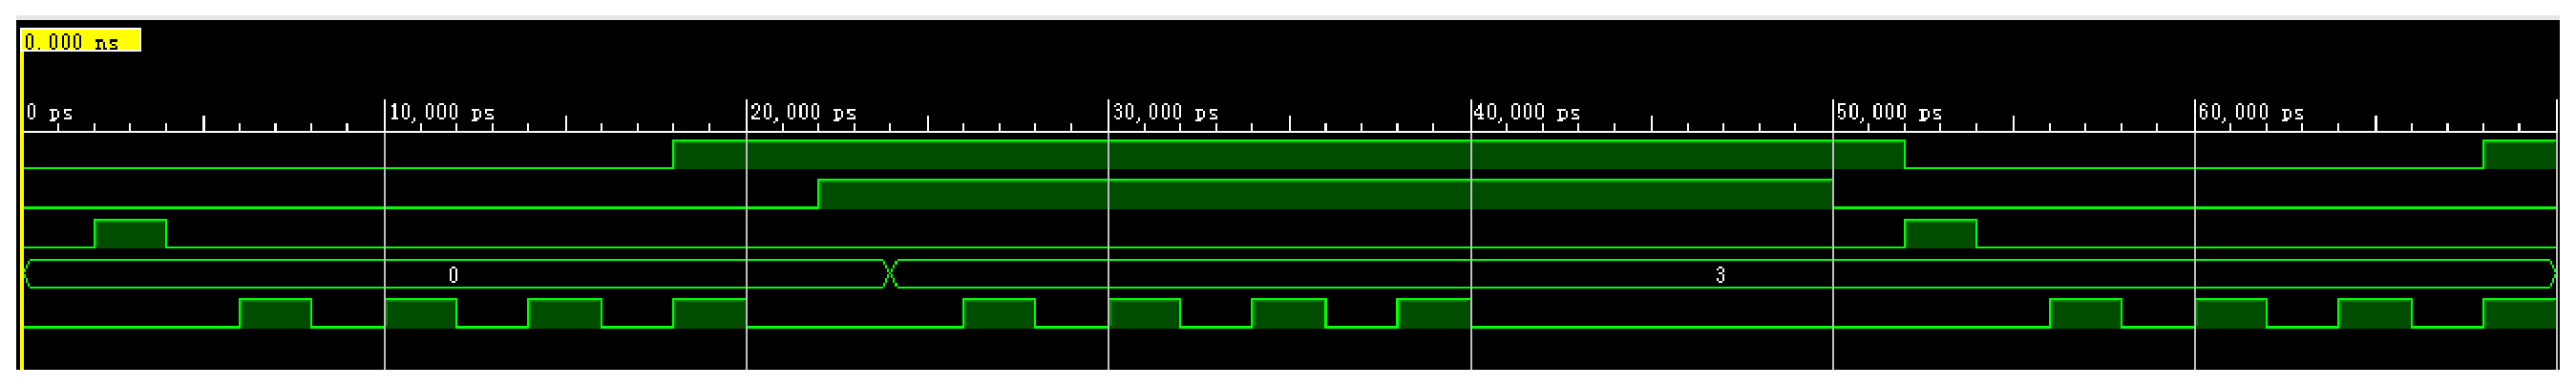
\includegraphics[width=0.9\textwidth]{./images/AlongSimOver.eps}

运行效果良好,开锁上锁,修改密码都做的相当不错。

\subsection{B部分仿真}
\paragraph{按键处理}
\begin{lstlisting}[language={verilog}]
module press_input_sim;
reg en2,s0,s1,s2,s3;
wire [1:0]out1,out2;
wire clk1,clk2;
press_input_n a(clk1,clk2,en2,out1,out2,s0,s1,s2,s3);
initial
begin
    en2=0;
    {s3,s2,s1,s0}=4'b0000;
    #100
    {s3,s2,s1,s0}=4'b0001;
    #100
    {s3,s2,s1,s0}=4'b0000;
    #100
    {s3,s2,s1,s0}=4'b0010;
    #100
    {s3,s2,s1,s0}=4'b0000;
end
endmodule

\end{lstlisting}
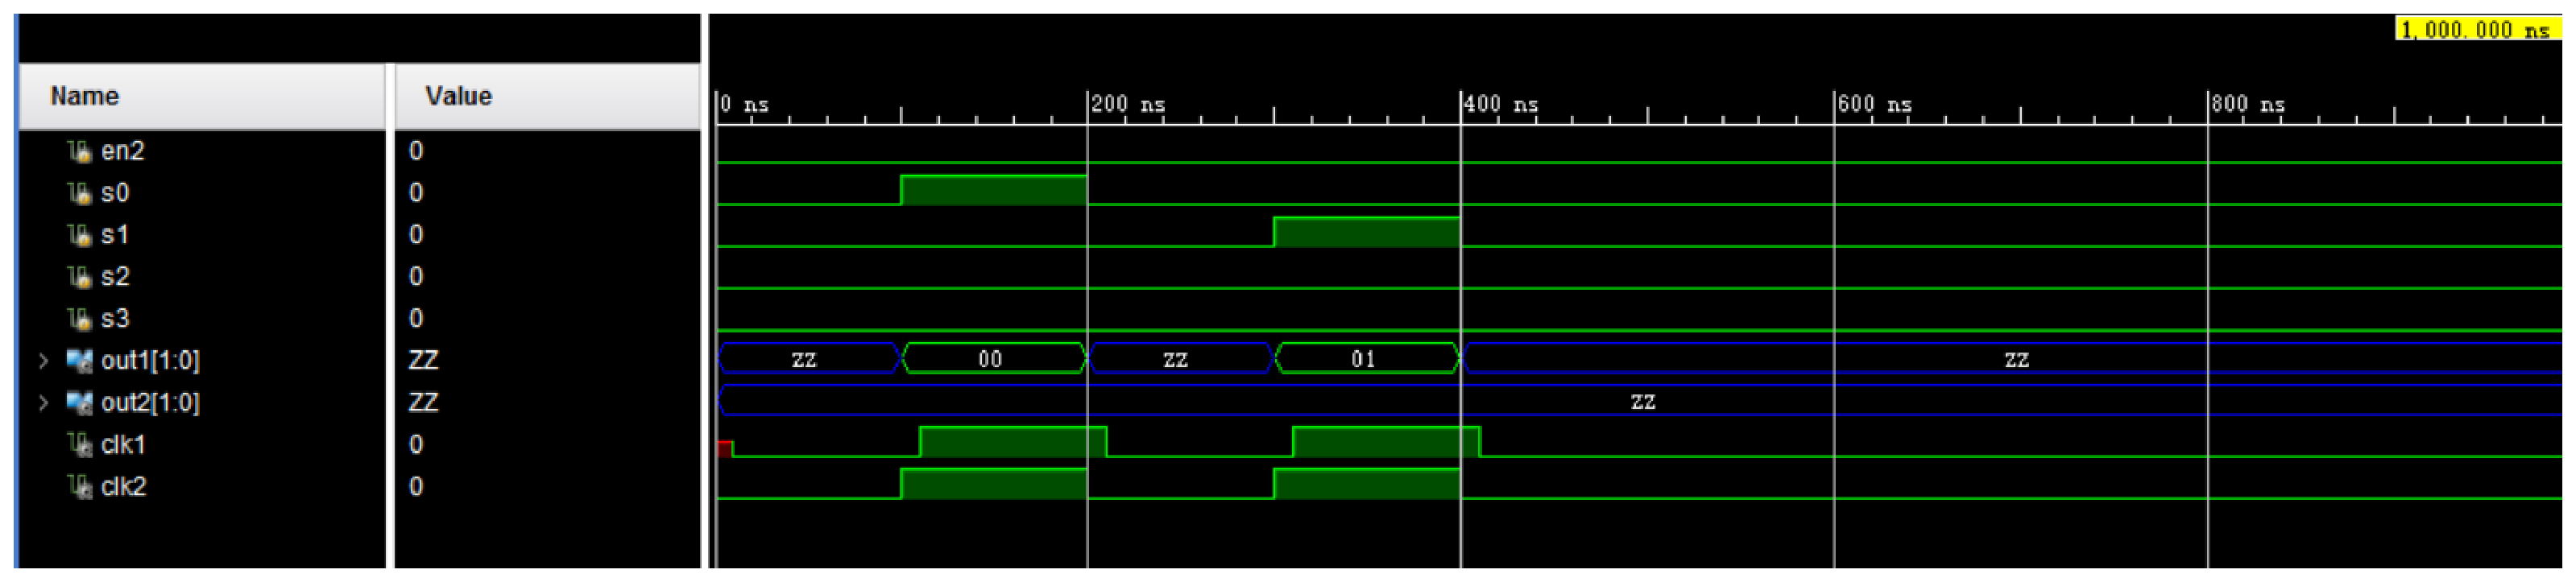
\includegraphics[width=0.9\textwidth]{./images/Lsim5.eps}

\paragraph{按键计数器}
\begin{lstlisting}[language={verilog}]
module press_counter_sim;
reg clk,clr;
wire a,b,c,d,e,f,g,q0,q1,q2,Z,time_counter_start;
press_counter_n my(Z,a,b,c,clk,clr,d,e,f,g,q0,q1,q2,time_counter_start);
initial
begin
    clr=0;
    clk=0;
    #10 clr=1;
end
always #40 clk=~clk;
endmodule

\end{lstlisting}
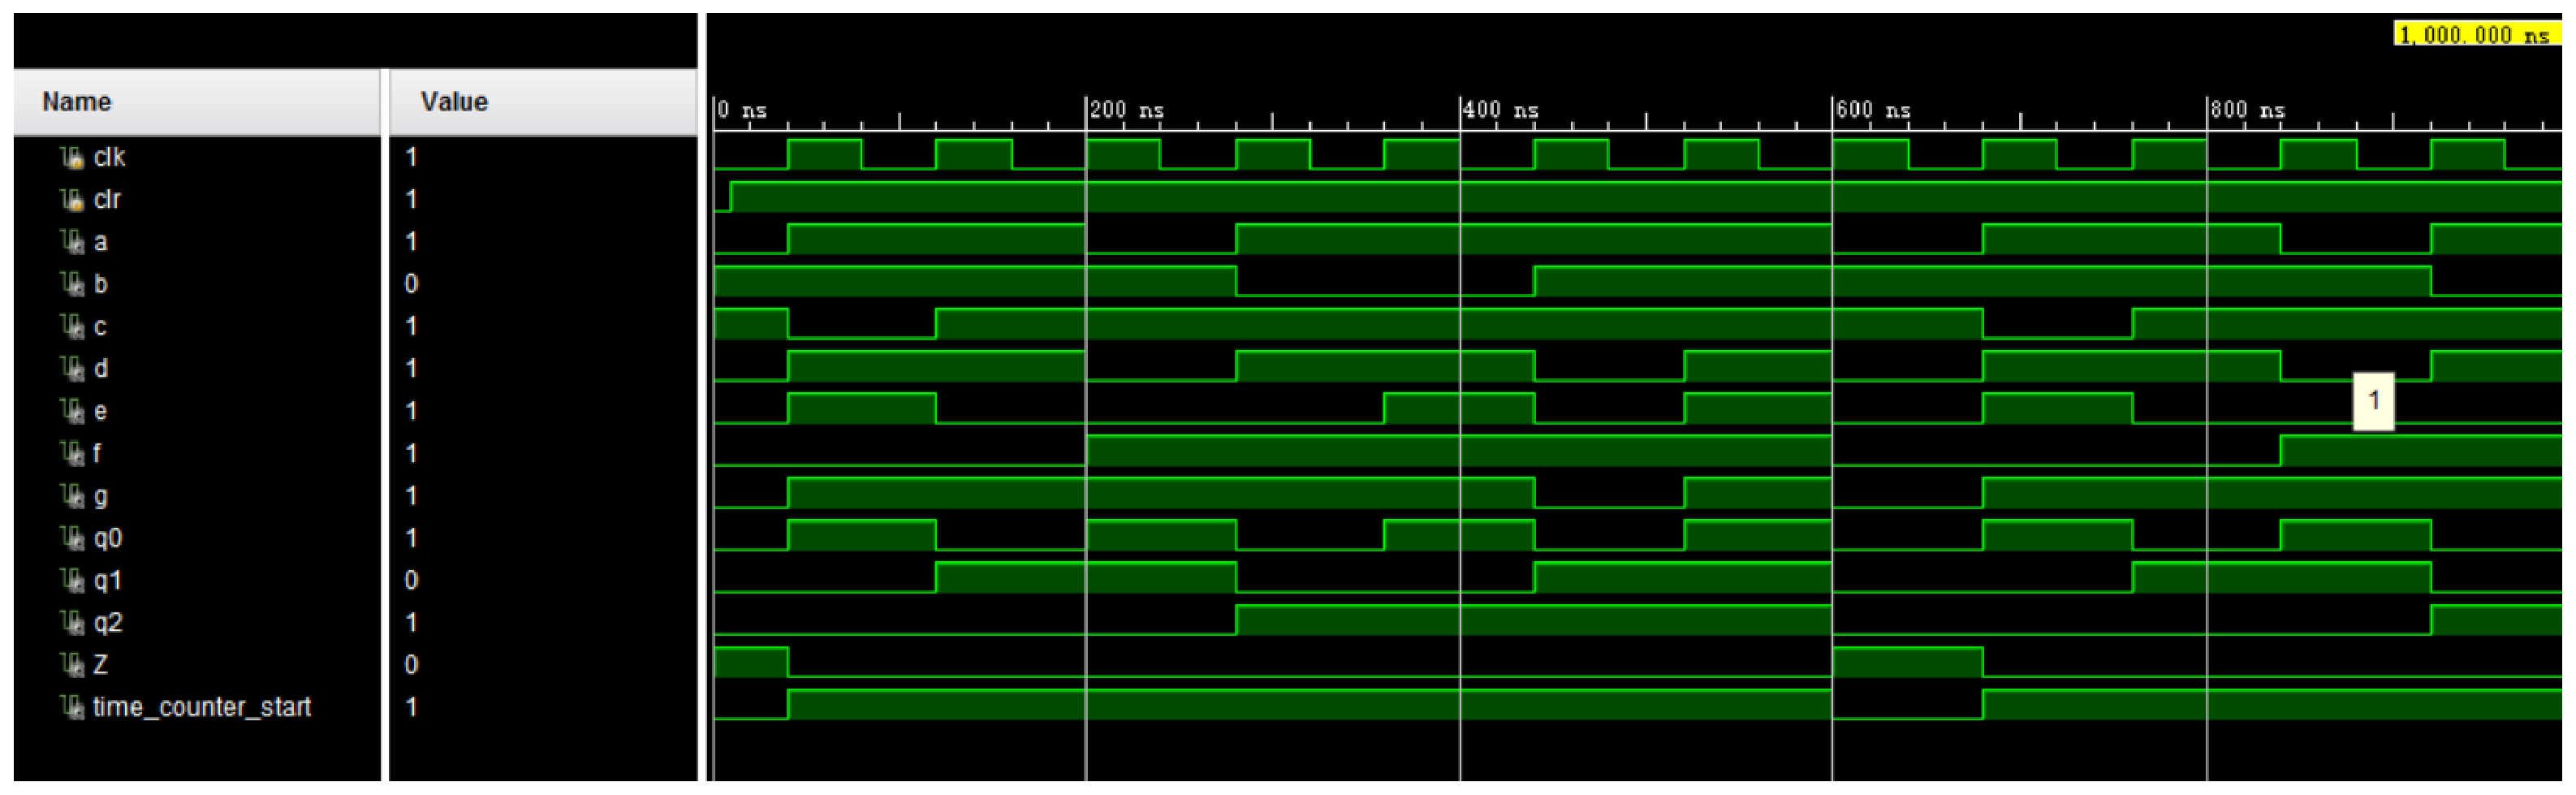
\includegraphics[width=0.9\textwidth]{./images/Lsim6.eps}

\paragraph{整体仿真}
\begin{lstlisting}[language={verilog}]
module lai_sim;
wire Z,a,b,c,d,e,f,g,q0,q1,q2,clk1,time_counter_start;
wire [6:0]s;
wire [1:0]out1,out2;
reg clr,en2,s0,s1,s2,s3;
lai lx
  (Z,a,b,c,clk1,clr,d,e,
    en2,f,g,out1,out2,q0,q1,
    q2,s0,s1,s2,s3,time_counter_start);
    initial
    begin
        clr=0;
        en2=0;
        s0=0;
        s1=0;
        s2=0;
        s3=0;
        #10 clr=1;
        #10 clr=0;
        #10 s1=1;
        #10 s1=0;//1
        #10 s0=1;
        #10 s0=0;//0
        #10 s0=1;
        #10 s0=0;//0
        #10 s0=1;
        #10 s0=0;//0
        #10 s0=1;
        #10 s0=0;//0
        #10 s0=1;
        #10 s0=0;//0
        #10 s0=1;
        #10 s0=0;//0
        #10 s0=1;
        #10 s0=0;//0
    end
endmodule

\end{lstlisting}

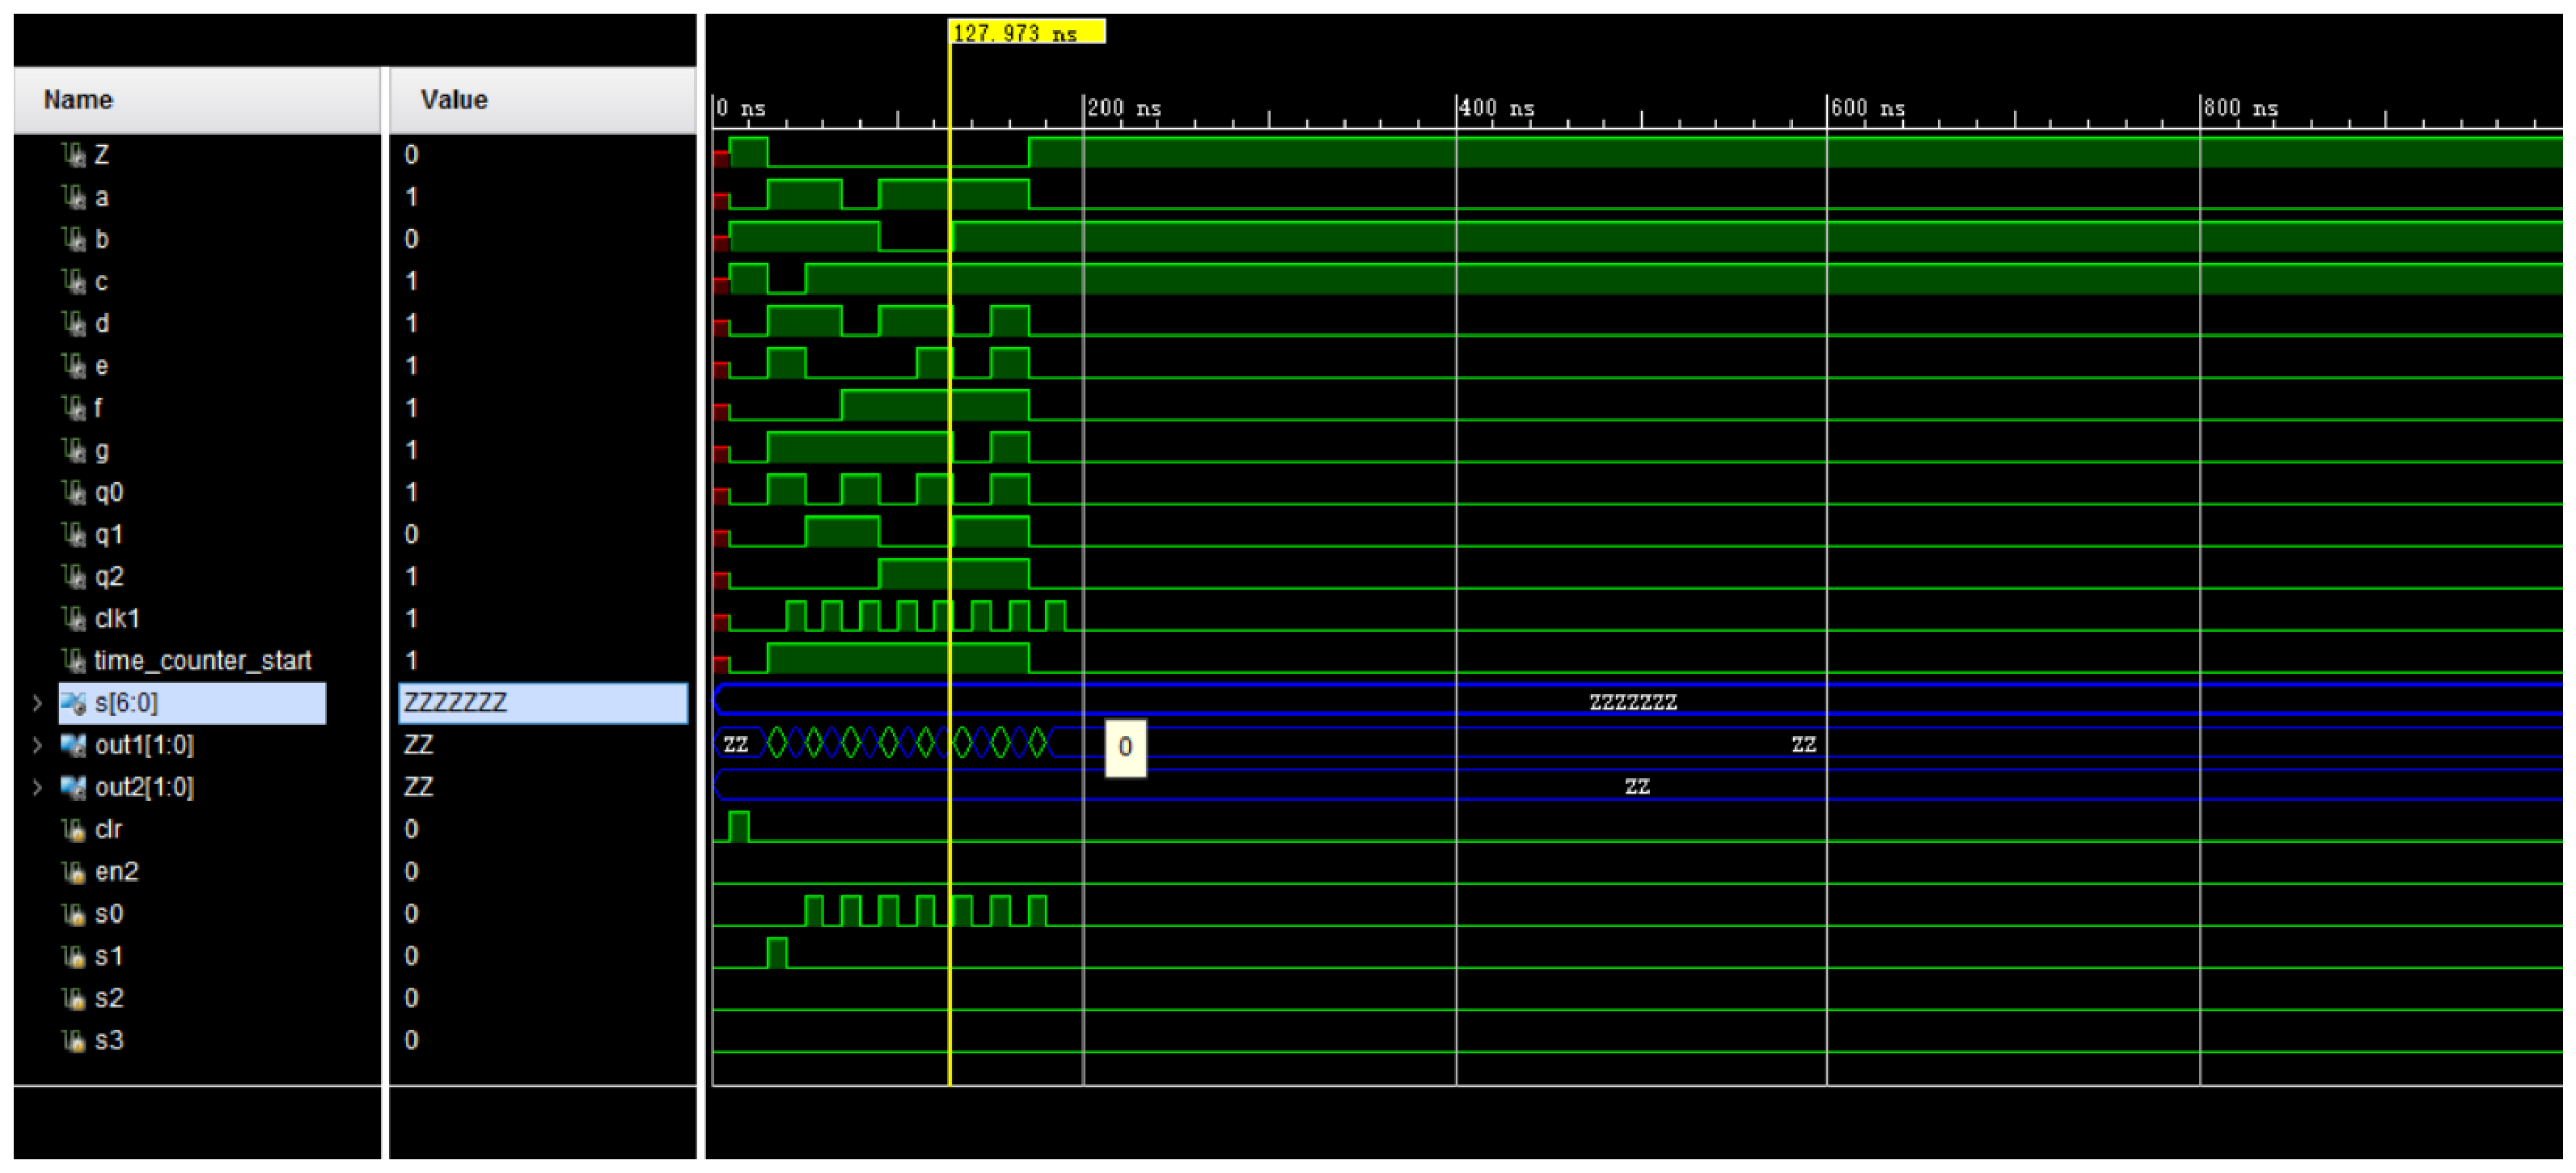
\includegraphics[width=0.9\textwidth]{./images/Lsim4.eps}


\section{工作说明}
\paragraph{冯云龙}密码处理,密码列表,密码计数器,开锁控制器,计时器,实验报告。
\subsection{密码处理}
\begin{lstlisting}[language={verilog}]
module pwdprocess(
    input [1:0] keypwd,             //按键输入密码
    input [1:0] cmppwd,             //正确密码
    input keypress,                 //按键脉冲,上升沿触发
    output res                      //输出计数脉冲
    );
    wire cmp;
    assign cmp=keypwd==cmppwd;
    assign res = cmp && keypress;
endmodule
\end{lstlisting}

\subsection{密码表}
\begin{lstlisting}[language={verilog}]
module pwdlist(
    input [2:0]toselect,        //计数选择
    output reg[1:0]currpwd,      //输出密码
    output reg[2:0]pwdlen,       //密码长度
    input change,             //是否修改密码
    input unlock,             //是否已解锁
    input [1:0]key,           //数据输入
    input keypress            //按键脉冲
    );
    reg [15:0]pwd;            //每两位是一组密码.
    reg [2:0]count;

    wire NClk;
    assign NClk = keypress && change && unlock;

    initial begin
    count = 0;
    pwd = 0;                  //初始密码
    pwdlen = 4;               //初始密码长度
    end

    always @(toselect,pwd)    //密码选择部分
    begin
    case(toselect)
    3'b000 : currpwd = pwd[1:0];
    3'b001 : currpwd = pwd[3:2];
    3'b010 : currpwd = pwd[5:4];
    3'b011 : currpwd = pwd[7:6];
    3'b100 : currpwd = pwd[9:8];
    3'b101 : currpwd = pwd[11:10];
    3'b110 : currpwd = pwd[13:12];
    3'b111 : currpwd = pwd[15:14];
    endcase
    end

    always @(posedge NClk)
    begin
    if(change && unlock) begin//已经解锁并且给了密码修改使能
    case(count)
    3'b000 : pwd[1:0] = key;
    3'b001 : pwd[3:2] = key;
    3'b010 : pwd[5:4] = key;
    3'b011 : pwd[7:6] = key;
    3'b100 : pwd[9:8] = key;
    3'b101 : pwd[11:10] = key;
    3'b110 : pwd[13:12] = key;
    3'b111 : pwd[15:14] = key;
    endcase
    count = count + 1;
    end
    else count = 0;
    end

    always @(negedge change)begin         //密码长度修改
    if(unlock) pwdlen = count;
    end

endmodule
\end{lstlisting}

\subsection{密码计数器}
\begin{lstlisting}[language={verilog}]
module counter(
    input CLK,                //计数时钟
    input CLR,                //复位
    output reg[2:0]num           //当前计数
    );
    initial num = 0;

    always @(posedge CLK) begin
    if(CLR)
      num = 0;
    else
      num = num + 1;
    end
endmodule
\end{lstlisting}
\subsection{开锁控制器}
\begin{lstlisting}[language={verilog}]
module Lock(
    input [2:0]count,              //当前输入正确的密码个数
    input [2:0]length,             //密码长度
    output state              //当前解锁状态,1为开锁
    );
    assign state = (count == length);
endmodule
\end{lstlisting}

\subsection{核心功能封装}
\begin{lstlisting}[language={verilog}]
module Along(
    input Change,                   //密码修改使能
    input KeyPress,                 //按键脉冲
    input [1:0]KeyValue,            //按键值
    input Lock_It,                  //上锁信号
    output LockState                //开锁状态
    );

      wire toLock;
      assign toLock=~Lock_It;

      wire [2:0]currlen;
      wire [1:0]currpwd;
      wire [2:0]pwdlen;
      wire isRight;

      Lock LockMgr
             (.count(currlen),
              .length(pwdlen),
              .state(LockState));
        counter PwdLen
             (.CLK(isRight),
              .CLR(toLock),
              .EN(LockState),
              .num(currlen));
        pwdlist Pwd_list
             (.change(Change),
              .currpwd(currpwd),
              .key(KeyValue),
              .keypress(KeyPress),
              .pwdlen(pwdlen),
              .toselect(currlen),
              .unlock(LockState));
        pwdprocess Process
             (.cmppwd(currpwd),
              .keypress(KeyPress),
              .keypwd(KeyValue),
              .res(isRight));
endmodule
\end{lstlisting}

\subsection{计时器}
\begin{lstlisting}[language={verilog}]
module TimeClock(
    input inClk,
    output outClk
    );
    reg [31:0]timeclk;

    assign outClk = timeclk[21];
    initial begin
    timeclk = 0;
    end

    always@(posedge inClk)begin
    timeclk = timeclk +1;
    end
endmodule
\end{lstlisting}
\begin{lstlisting}[language={verilog}]
module TimeShow(
    input show,                 //显示切换信号
    input clk,                  //时钟信号
    input pause,                //暂停计时
    input clr,                  //清零段
    output full,                //进位信号
    output reg sm_bit,          //片选信号
    output reg[6:0]sm_seg       //显示数码管
    );

    reg [3:0]timesec0;
    assign full = timesec0 == 4;

    initial begin
    sm_bit=1;
    sm_seg=1;
    timesec0=0;
    end

    always @(posedge clk or negedge clr) begin
    if(~clr)
      timesec0 = 0;
    else
    if(pause)begin
        if(timesec0==4)
        timesec0=0;
        else
        timesec0=timesec0+1;
        end
    end

    always@(posedge show)
    begin
    case(timesec0)
                0:sm_seg= 7'b0110011;                     //显示4
                1:sm_seg= 7'b1111001;                      //显示3
                2:sm_seg= 7'b1101101;                     //显示2
                3:sm_seg= 7'b0110000;                     //显示1
                4:sm_seg= 7'b1111110;                     //显示0
                default:
                sm_seg= 7'b0000000;                        //不显示
    endcase
    end
endmodule
\end{lstlisting}

\paragraph{赖昕}按键计数器,按键译码处理器,显示器,最终组装。

\subsection{D触发器}
\begin{lstlisting}[language={verilog}]
module dff(clk,clr,d,q);//d触发器
input clk,clr,d;
//clk:时钟沿(上升沿触发)
//clr:异步清零端(低电平有效)
//d:触发器输入值端
output q;//q:触发器输出端
reg q;
always@(posedge clk or negedge clr)//clk上升沿触发,clr异步
begin
if(~clr) q<=0;//clr低电平有效
else if(clk) q<=d;//来时钟沿时,q=d;
end
endmodule

\end{lstlisting}
\subsection{4-2编码器}
\begin{lstlisting}[language={verilog}]
module encoder4_2(en1,en2,s0,s1,s2,s3,out1,out2);
input en1,en2;//en1:译码器使能端;en2:修改密码使能端
input s0,s1,s2,s3;//s0~s3;按键输入
output [1:0]out1;//out1:用于输入密码的输出
output [1:0]out2;//out2:用于修改密码的输出
reg [1:0]out1;
reg [1:0]out2;
always@(*)
begin
    if(~en1)//如果en1为低电位,则输出均为高阻态
    begin
        out1=2'bzz;
        out2=2'bzz;
    end
    else if(~en2)
    //如果en1为高电位且en2为低电位,
    //则输入密码out1输出为编码输出,修改密码out2输出为高阻态
    begin
        out2=2'bzz;
        case({s3,s2,s1,s0})
            4'b0001:out1=2'b00;
            4'b0010:out1=2'b01;
            4'b0100:out1=2'b10;
            4'b1000:out1=2'b11;
        endcase
    end
    else 
    //如果en1为高电位且en2为高电位,
    //则修改密码out2输出为编码输出,输入密码out1输出为高阻态
    begin
        out1=2'bzz;
        case({s3,s2,s1,s0})
            4'b0001:out2=2'b00;
            4'b0010:out2=2'b01;
            4'b0100:out2=2'b10;
            4'b1000:out2=2'b11;
        endcase
    end
end
endmodule
\end{lstlisting}
\subsection{移位寄存器}
\begin{lstlisting}[language={verilog}]
module shift_register(clk,I,O);
input I,clk;
output O;
reg [3:0]b;
wire O;
always@(posedge clk)//当时钟上升沿来到时,寄存器移位。
begin
    b<={b[2:0],I};
end
assign O=b[3];
endmodule
\end{lstlisting}

\subsection{按键处理}
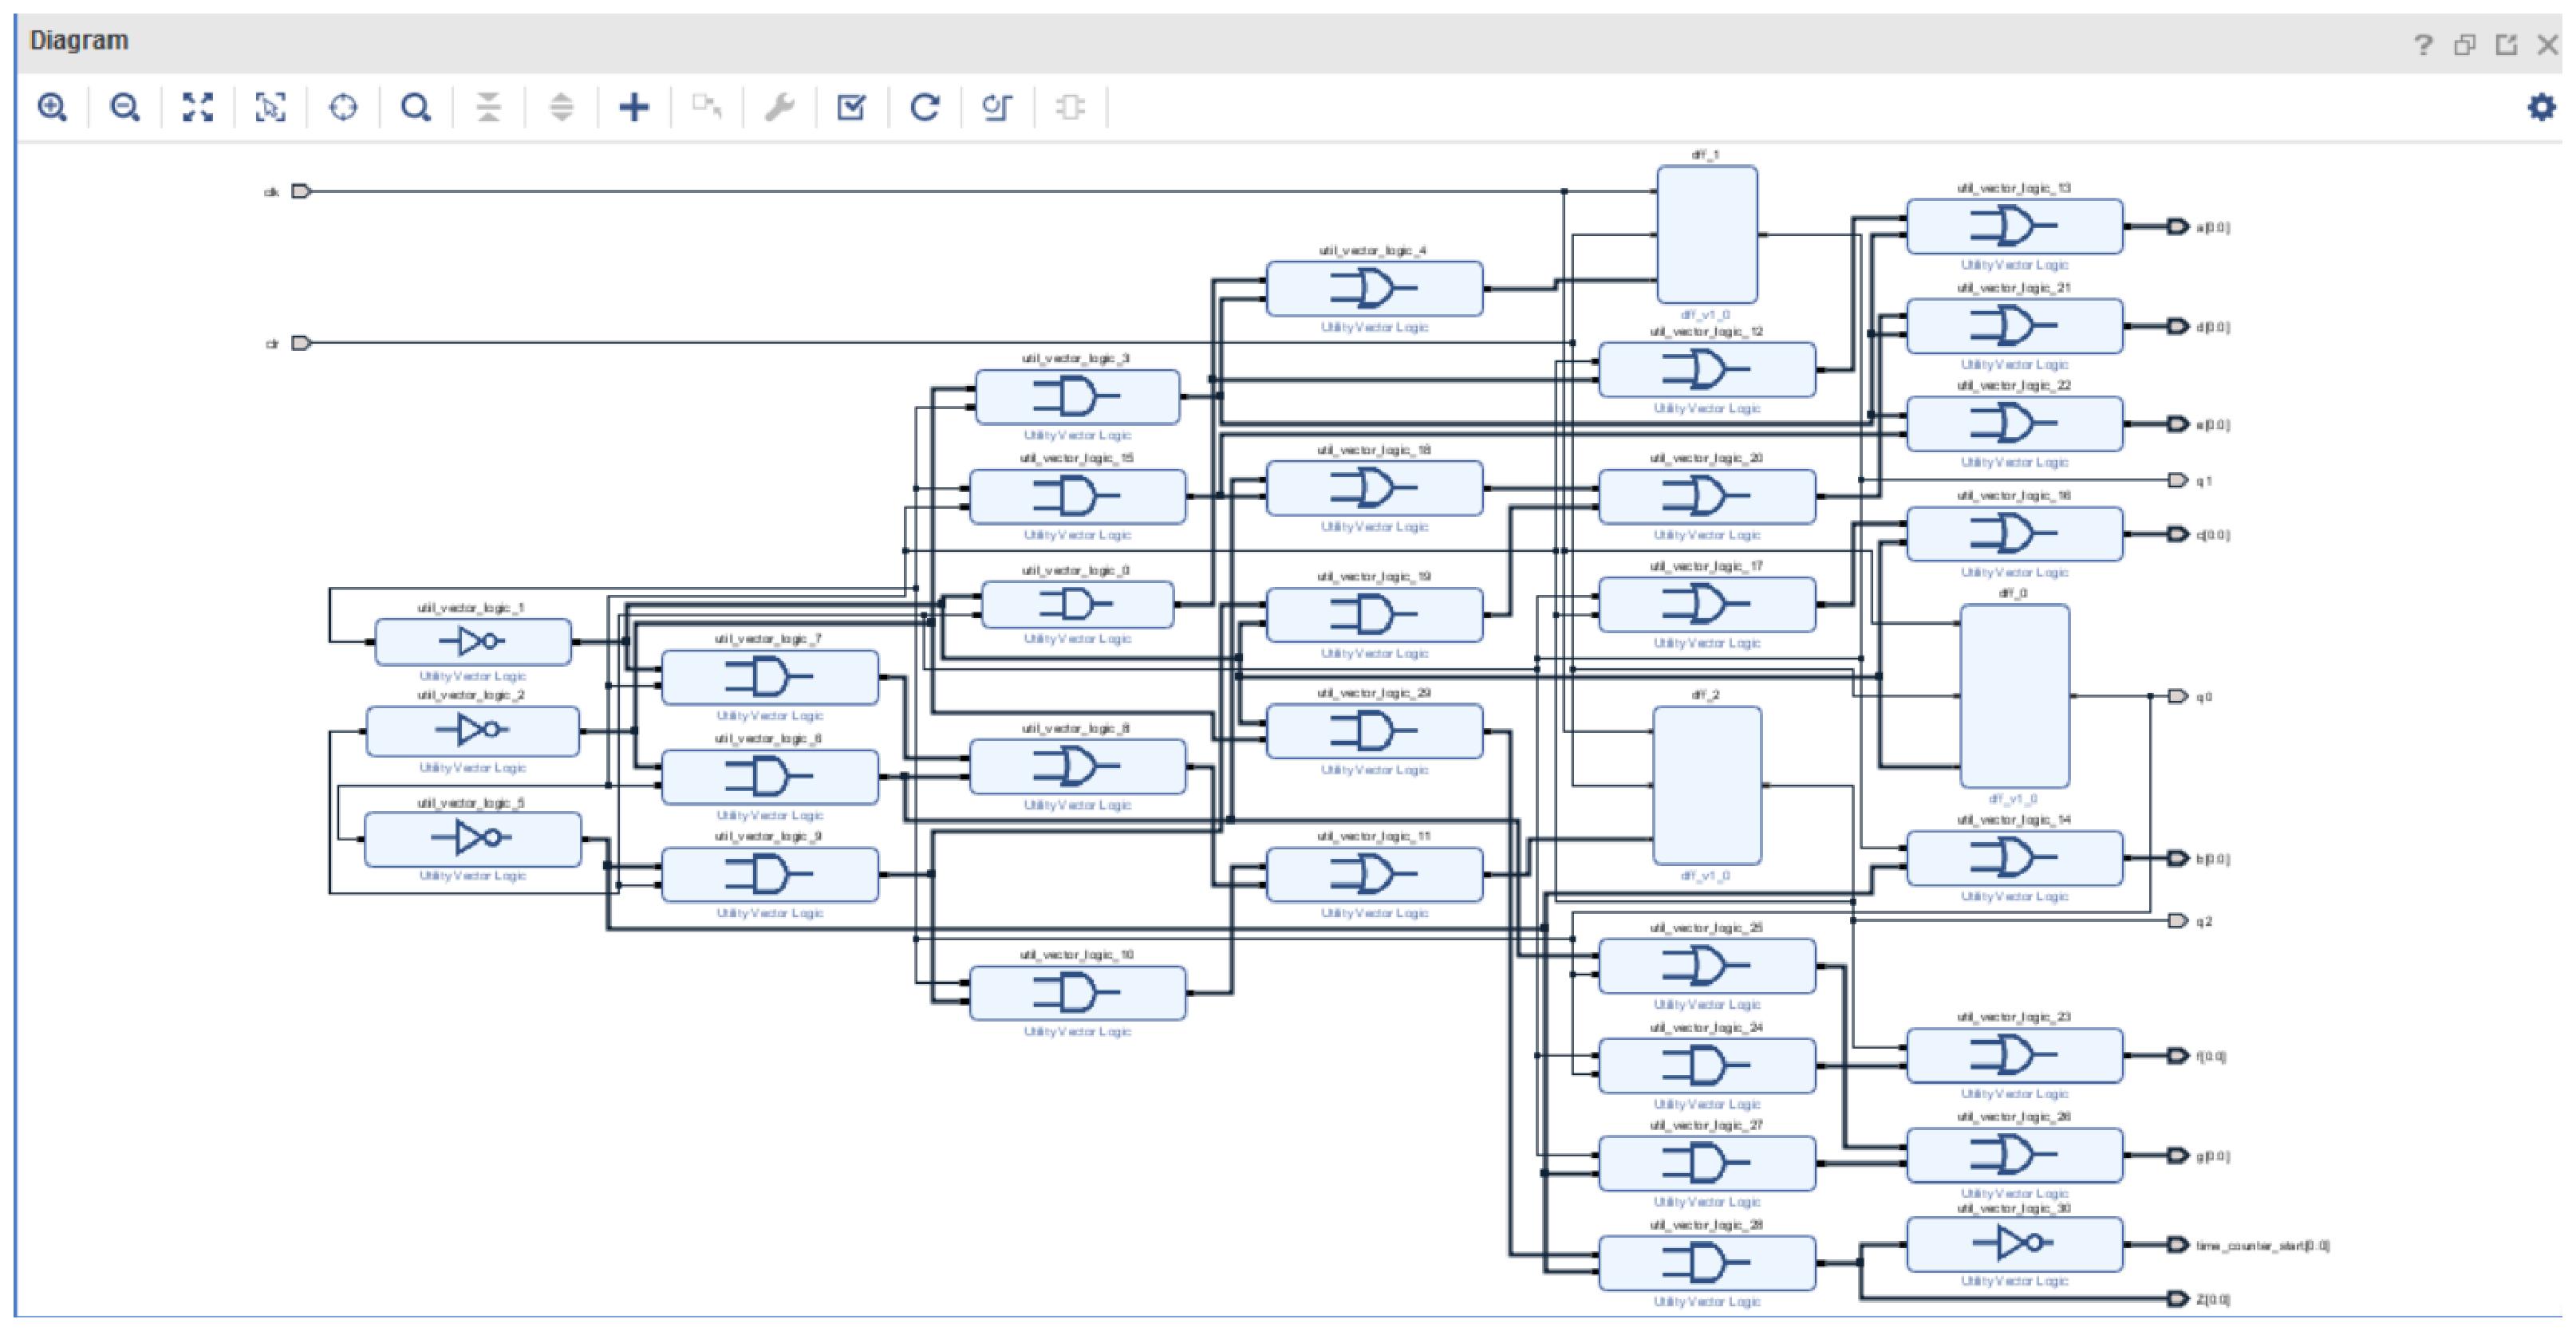
\includegraphics[width=0.9\textwidth]{./images/block1.eps}
\subsection{按键计数器}
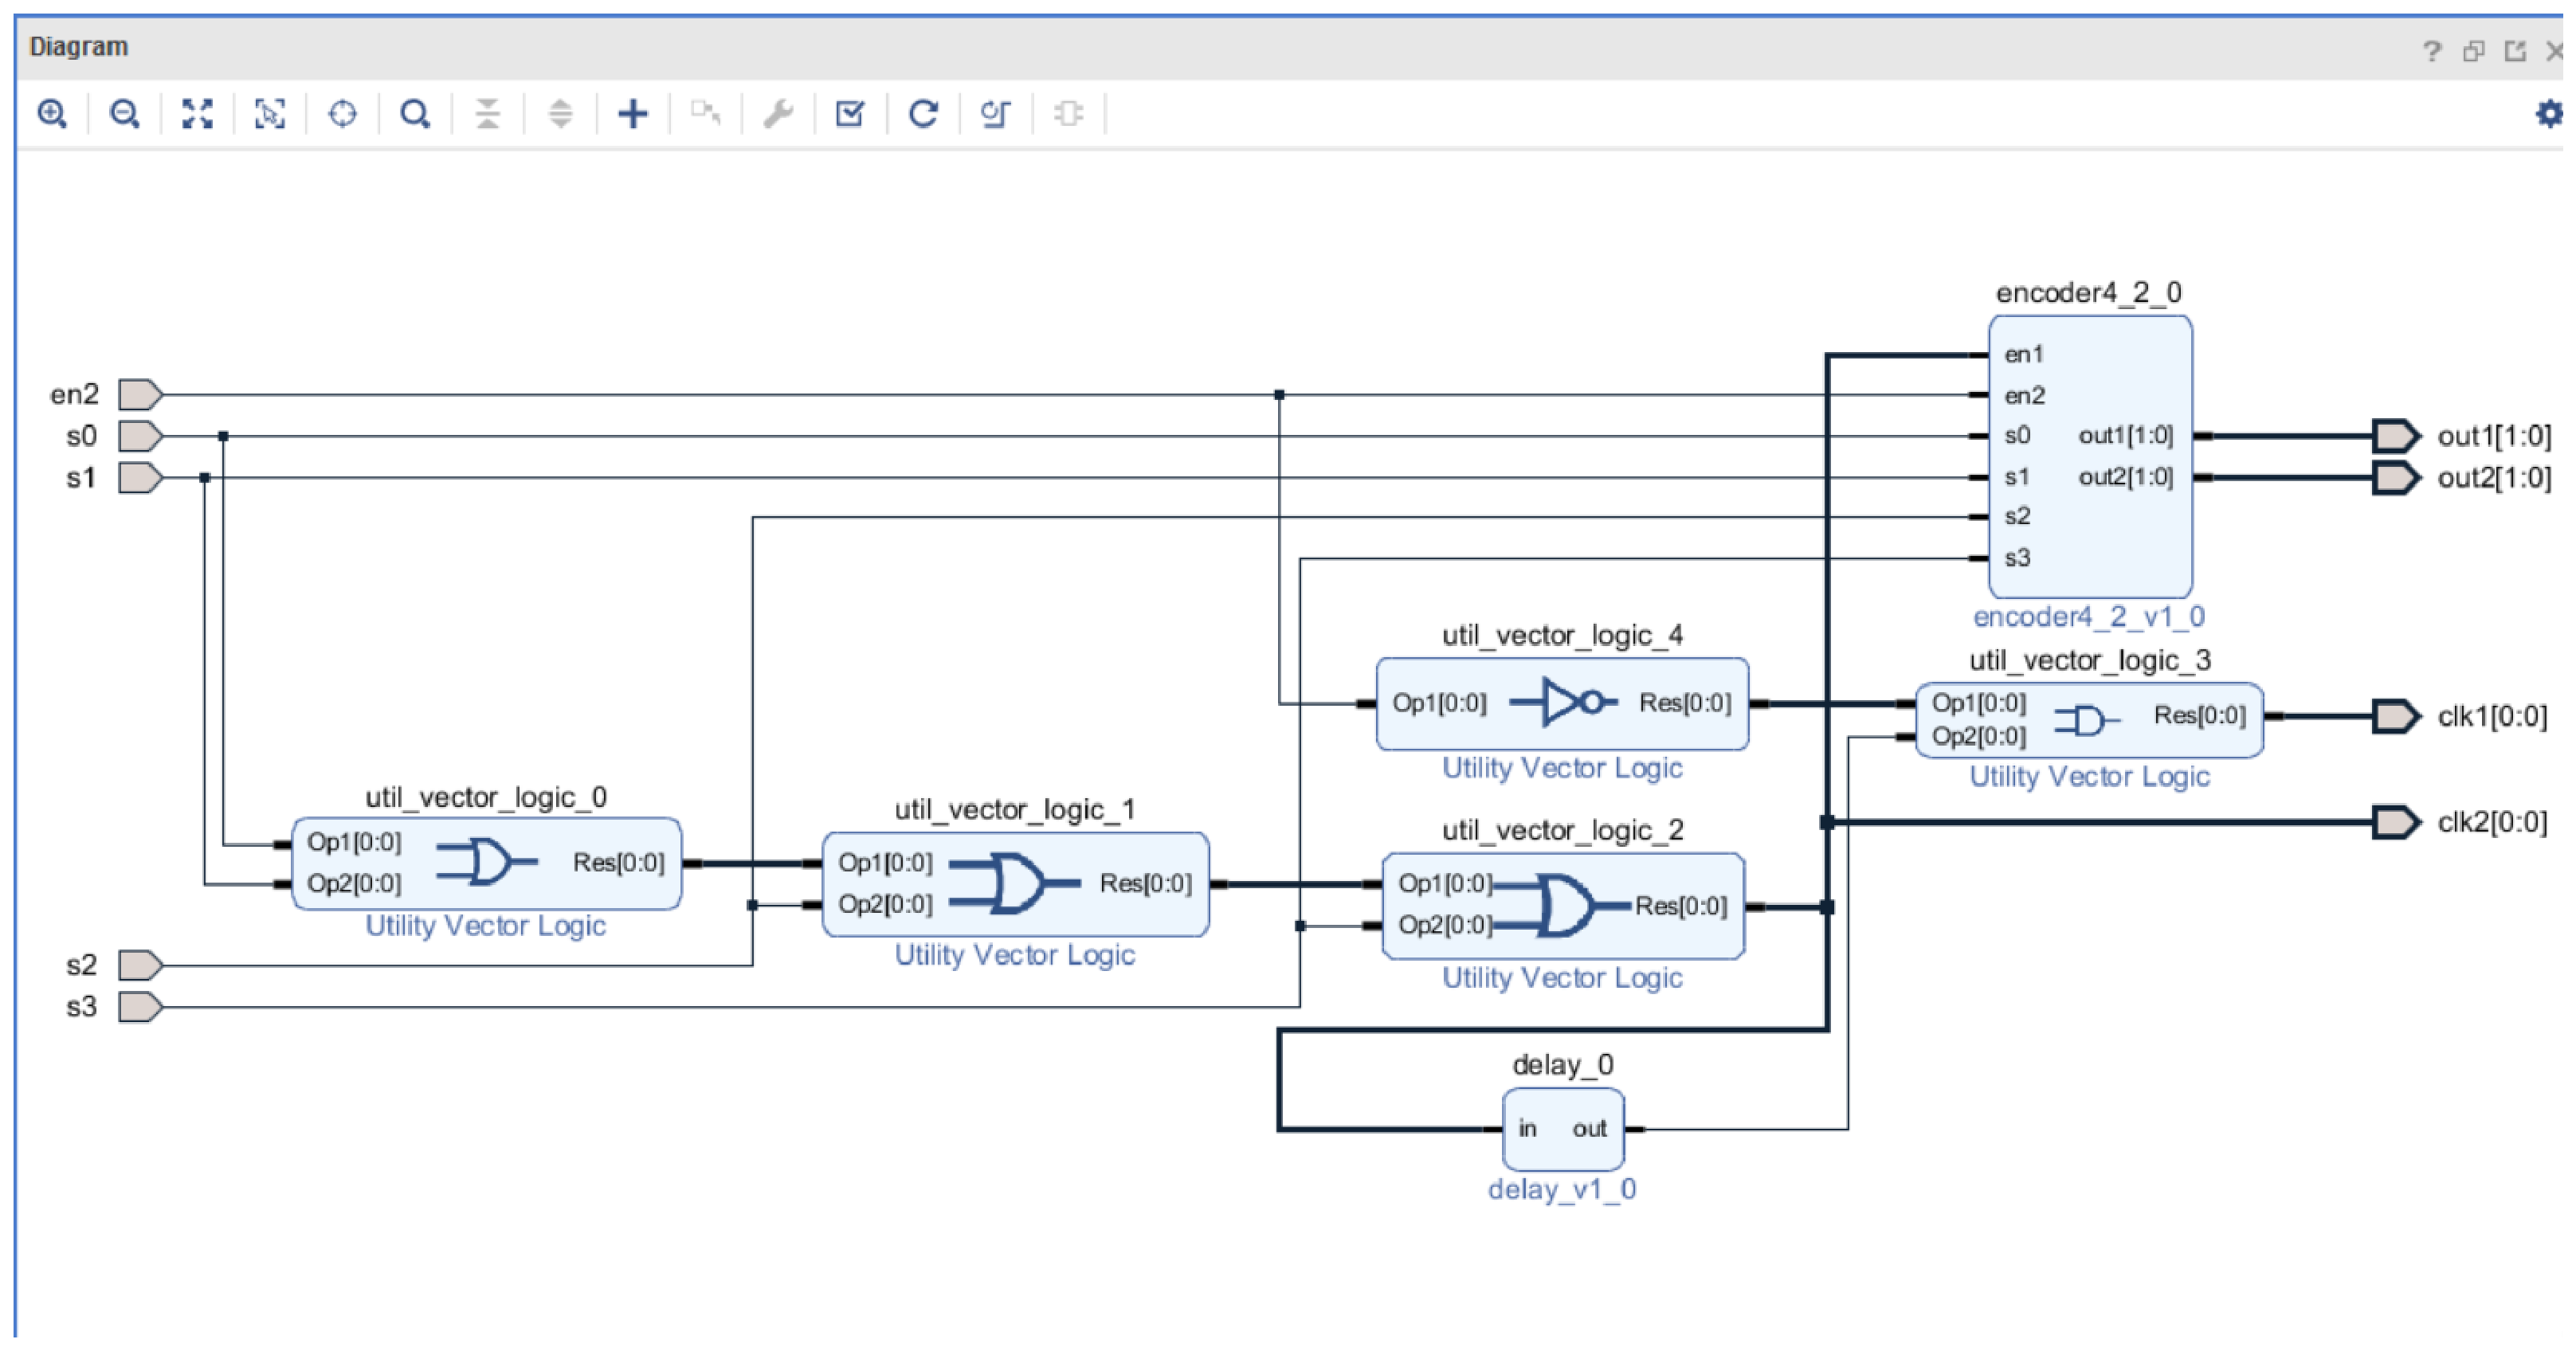
\includegraphics[width=0.9\textwidth]{./images/block2.eps}
\end{document} 